\documentclass{article}

% if you need to pass options to natbib, use, e.g.:
\PassOptionsToPackage{numbers, compress}{natbib}
% before loading neurips_2024


% ready for submission
\usepackage[final]{neurips_2024}


% to compile a preprint version, e.g., for submission to arXiv, add add the
% [preprint] option:
%     \usepackage[preprint]{neurips_2024}


% to compile a camera-ready version, add the [final] option, e.g.:
%     \usepackage[final]{neurips_2024}


% to avoid loading the natbib package, add option nonatbib:
%    \usepackage[nonatbib]{neurips_2024}


\usepackage[utf8]{inputenc} % allow utf-8 input
\usepackage[T1]{fontenc}    % use 8-bit T1 fonts
\usepackage{hyperref}       % hyperlinks
\usepackage{url}            % simple URL typesetting
\usepackage{booktabs}       % professional-quality tables
\usepackage{amsfonts}       % blackboard math symbols
\usepackage{nicefrac}       % compact symbols for 1/2, etc.
\usepackage{microtype}      % microtypography
\usepackage{xcolor}         % colors
\usepackage{algorithm}
\usepackage{algorithmic}
\usepackage{amsmath}
\usepackage{multicol}
\usepackage{natbib}
\usepackage{graphicx}
\usepackage{caption}
\usepackage{listings}
\lstset{
    showspaces=false,
    showstringspaces=false,
    showtabs=false
}

\title{Where Did It All Go Wrong? A Hierarchical Look into Multi-Agent Error Attribution}


% The \author macro works with any number of authors. There are two commands
% used to separate the names and addresses of multiple authors: \And and \AND.
%
% Using \And between authors leaves it to LaTeX to determine where to break the
% lines. Using \AND forces a line break at that point. So, if LaTeX puts 3 of 4
% authors names on the first line, and the last on the second line, try using
% \AND instead of \And before the third author name.

% \author{
%   Adi Banerjee* \\
%   Amazon Web Services \\
%   New York, NY, USA \\
%   \texttt{adibaner@amazon.com} \\
%   \AND
%   Ani Nair* \\
%   Amazon Web Services \\
%   Boston, MA, USA \\
%   \texttt{rianina@amazon.com} \\
% }
\author{
    Adi Banerjee$^*$ \\
    Amazon Web Services \\
    New York, NY, USA \\
    \texttt{adibaner@amazon.com} \And
    Anirudh Nair$^*$ \\
    Amazon Web Services \\
    Boston, MA, USA \\
    \texttt{rianina@amazon.com} \And
    Tarik Borogovac \\
    Amazon Web Services \\
    Boston, MA, USA \\
    \texttt{tarikbo@amazon.com}
}

% \renewcommand{\thefootnote}{\fnsymbol{footnote}}
% \footnotetext[1]{Equal Contribution.}
% \renewcommand{\thefootnote}{\arabic{footnote}}

% \def\equalcontrib{$^*$Equal contribution}
% \date{\vspace{1em}\textit{\equalcontrib}}

\begin{document}
\maketitle
\def\thefootnote{*}\footnotetext{Equal Contribution.}\def\thefootnote{\arabic{footnote}}

\begin{abstract}
  Error attribution in Large Language Model (LLM) multi-agent systems presents a significant challenge in debugging and improving collaborative AI systems. Current approaches to pinpointing agent and step level failures in multi-agent interaction traces\textemdash whether using all-at-once evaluation, step-by-step analysis, or binary search\textemdash fall short when analyzing complex patterns, struggling with both accuracy and consistency. We present ECHO (Error attribution through Contextual Hierarchy and Objective consensus analysis), a novel algorithm that combines hierarchical context representation, objective analysis-based evaluation, and consensus voting to improve error attribution accuracy. Our approach leverages a positional-based leveling of contextual understanding while maintaining objective evaluation criteria, ultimately reaching conclusions through a consensus mechanism. Experimental results demonstrate that ECHO outperforms existing methods across various multi-agent interaction scenarios, showing particular strength in cases involving subtle reasoning errors and complex interdependencies. Our findings suggest that leveraging these concepts of structured, hierarchical context representation combined with consensus-based objective decision-making, provides a more robust framework for error attribution in multi-agent systems.

  %While existing approaches attempt to identify the responsible agent and critical error step in interaction traces, they often struggle with accuracy and reliability. Current methods, including all-at-once evaluation, step-by-step analysis, and binary search strategies, face limitations in handling complex interaction patterns and maintaining consistency in their attributions. 

\end{abstract}

% \thanks{\textsuperscript{*}These authors contributed equally to this work.}

\section{Introduction}

% The evolution of large language models (LLMs) has led to their implementation as collaborative, specialized agents working together in structured systems \cite{guo2024large, li2025review}. Rather than relying on individual agents, these systems break down complex challenges into manageable components, distributing them among purpose-specific agents who work in concert to achieve common objectives \cite{chen2024internet, li2023camel}. This coordinated approach demands effective orchestration of various agents, each with their own specialized functions and duties. The development of these collaborative systems requires careful consideration of interconnected graph structures that map out how agents relate to and depend on each other, how information flows between them, and what logical constraints govern their interactions. These structural elements serve as the cornerstone for building expandable and flexible multi-agent frameworks\cite{zhou2025multi}.

The evolution of large language models (LLMs) has driven their implementation as collaborative, specialized agents working together in structured systems \cite{guo2024large, li2025review}. These systems break down complex challenges into manageable components, distributing them among purpose-specific agents that work in concert toward common objectives \cite{chen2024internet, li2023camel}. Such coordination demands effective orchestration, with each agent performing specialized functions. Building these collaborative systems requires careful consideration of interconnected graph structures\textemdash mapping agent relationships, information flows, and logical constraints. These structural elements form the foundation for expandable and flexible multi-agent frameworks \cite{zhou2025multi}.

% While these Multi-Agent Systems (MASs) have demonstrated remarkable task performance in domains such as coding \cite{hong2023metagpt}, medical QA \cite{kim2024mdagents}, and financial decision-making \cite{yu2024fincon}, their multi-step nature makes them susceptible to compounding errors: a mistake in an earlier agent amplifies mistakes in subsequent steps and can derail the system entirely. As a result, attributing the initial error to the appropriate agent and step in multi-turn chains becomes paramount to mitigating such mistakes and further improving the MASs. 

Multi-Agent Systems (MASs) have demonstrated remarkable performance across use-cases such as coding \cite{hong2023metagpt}, medical QA \cite{kim2024mdagents}, and financial decision-making \cite{yu2024fincon}. However, their multi-step nature makes them vulnerable to compounding errors, where early mistakes amplify through subsequent steps and can derail the entire system. As a result, identifying the initial error's source—both agent and step—becomes crucial for mitigating such failures and improving these systems.

% Manual error attribution becomes unscalable as MASs grow in size and complexity, necessitating an automated approach. However, according to the Who\&When dataset and benchmark \cite{zhang2025agent}, even state-of-the-art (SOTA) closed-source LLMs (such as OpenAI's GPT-4o \cite{hurst2024gpt} and o1 \cite{jaech2024openai}) and open-source LLMs (such as Llama 4 models \cite{meta2025llama}) struggle with this task. The complexity arises from several factors: (1) interdependent nature of agent interactions; (2) potentially large context sizes; and (3) the necessity to understand both local and global context within the interaction trace. Traditional debugging approaches often fall short when applied to these dynamic systems where errors may be subtle and context-dependent.

As MASs grow in complexity, manual error attribution becomes unscalable, necessitating an automated approach. However, according to the Who\&When benchmark \cite{zhang2025agent}, even SOTA LLMs\textemdash both closed-source (GPT-4o \cite{hurst2024gpt}, o1 \cite{jaech2024openai}) and open-source (Llama 4 \cite{meta2025llama})\textemdash struggle with this task. The complexity stems from interdependent agent interactions, large context sizes, and the need to understand both local and global context within interaction traces. Traditional debugging approaches falter in these dynamic systems where errors are often subtle and context-dependent.

% However, when these systems fail, the ability to identify the root causes of failure is a crucial problem. This challenge of determining which agents and more specifically, which steps caused the critical error - represents a significant obstacle in debugging and improving multi-agent systems.

% Intuitive approaches to automated error attribution in LLM-based MAS have revolved around different levels of exposure to failure logs. For example, all-at-once approaches provide error-identifying LLMs with the complete failure log simultaneously, requesting identification of both the responsible agent and the critical error step. Alternatively, step-by-step methods present the failure log sequentially, allowing the LLM to evaluate each interaction incrementally until an error is detected. More sophisticated binary search approaches iteratively narrow down the error location by halving interaction traces at every step, and having the LLM determine which half contains the critical mistake.

Automated error attribution in LLM-based MAS has explored varying approaches to failure log analysis. For example, all-at-once methods expose LLMs to complete logs simultaneously for agent and step identification \cite{zhang2025agent}. Alternatively, step-by-step approaches evaluate interactions sequentially until detecting an error \cite{zhang2025agent}. More sophisticated binary search methods iteratively narrow the search space by having LLMs determine which half of the trace contains the critical mistake \cite{zhang2025agent}.

This paper presents ECHO (Error attribution through Contextual Hierarchy and Objective consensus analysis), a novel approach to error attribution in multi-agent systems, that addresses these limitations, by guiding error attribution through developing a hierarchical context representation of the entire interaction trace, providing independent objective analyses across these contexts and cross-validating their findings via consensus voting.

%TODO: MOVE TO FUTURE WORK - DONE
% The ability to do accurate multi-scale dependency reasoning trace error analysis and attribution can have important consequences to development of AI. For reinforcement learning of reasoning models, even though the reasoning traces used in training did converge to verifiable good answers, they may still contain false steps and noise. Those false steps and noise may reduce efficacy of the resulting model, by introducing extra false and distracting reasoning steps at test time, and can in turn contribute to loss of task coherence. Similarly, for single-agent optimization in AI system design, the ability to call out key errors in traces improves the identification of which part of the system prompt should be modified, potentially benefiting  feedback schemes such as GEPA \cite{agrawal2025gepareflectivepromptevolution} and DEEVO \cite{nair2025tournamentpromptsevolvingllm}.

\section{Related Work}

% \subsection{LLM as a Judge}
% Much research focus has gone into the automated evaluation of LLMs on various tasks \cite{fu2023gptscore,liu2023g,li2023alpacaeval}. 
\subsection{Evaluation of LLM Agents}
% Much research focus has gone into the automated evaluation of LLMs on various tasks \cite{fu2023gptscore,liu2023g,li2023alpacaeval}. However, more recent evaluation efforts revolve around the agentic capabilities of LLMs. AgentBench \cite{liu2023agentbench} evaluates LLMs' task completion abilities across diverse environments, including online shopping and house holding. MLAgentBench \cite{huang2023mlagentbench} tests if LLM agents can perform machine learning experimentation effectively. Another notable example is AssistantBench \cite{yoran2024assistantbench} which contains web-tasks that are realistic and time-consuming on nature and often require multi-turn web calls to solve. Agent-as-a-Judge \cite{zhuge2024agent} employs an LLM agent as the judge itself to evaluate other LLM agents by interacting with the available tools. ToolFormer \cite{schick2023toolformer}, AnyTool \cite{du2024anytool}, and ToolBench \cite{qin2023toolllm} all provide benchmarks on evaluating how well LLMs perform tool-use as API calling. As LLMs interact and invoke each other, evaluation frameworks have expanded to consider multi-agent scenarios. MultiAgentBench \cite{zhu2025multiagentbench} explicitly measures both coordination dynamics and competitive interactions, highlighting the unique challenges of mult-iagent environments. SwarmBench \cite{ruan2025benchmarking} evaluates the swarm intelligence capabilities of multi-agent systems through coordination tasks like foraging and flocking. 
Much research has focused on automated LLM evaluation across various tasks \cite{fu2023gptscore,liu2023g,li2023alpacaeval}, with recent efforts shifting toward assessing the agentic abilities of LLMs. AgentBench \cite{liu2023agentbench} tests task completion across environments like online shopping and householding, while MLAgentBench \cite{huang2023mlagentbench} evaluates LLM agents' abilities to perform machine learning experimentation. Similarly, AssistantBench \cite{yoran2024assistantbench} features realistic, time-intensive web tasks requiring multi-turn interactions, while Agent-as-a-Judge \cite{zhuge2024agent} leverages LLM agents to evaluate other agent peers through tool interactions. Finally, ToolFormer \cite{schick2023toolformer}, AnyTool \cite{du2024anytool}, and ToolBench \cite{qin2023toolllm} benchmark LLMs' API-calling capabilities via tool-use. As LLM agent interactions evolve, evaluation frameworks now address multi-agent scenarios: MultiAgentBench \cite{zhu2025multiagentbench} measures coordination and competitive dynamics, while SwarmBench \cite{ruan2025benchmarking} assesses swarm intelligence through coordination tasks like foraging and flocking.

\subsection{Error Attribution}
% The paradigm of error attribution of LLM outputs are closely related to evaluation of LLMs, but while evaluation typically measures task completion and output quality, error attribution focuses on systematically classifying the types and patterns of errors that occur to understand the fundamental failure modes of these models \cite{xu2025diagnosing, yin2022seq2seq, jiang2023tigerscore, ladhak2022contrastive}. ReaLMistake \cite{kamoi2024evaluating} categorizes assessable errors to test how proficient LLMs are at attributing errors in generated output. SynCheck \cite{wu2024synchronous} uses decoding dynamics to determine whether a generated sentence is trustworthy and backtracks if generated sentence is deemed to be unfaithful to some given text. In Self-Backtracking \cite{yang2025step}, a language model localizes errors in it own reasoning steps and backtracks and is then supervised fine-tuned on such traces to learn to backtrack during inference. Similarly, Process Reward Models (PRMs) \cite{lightman2023let} are trained via process annotation to evaluate the correctness of intermediate reasoning steps. Furthermore, ProcessBench \cite{zheng2024processbench} evaluates how capable PRMs are at identifying step-wise correctness. However, such methods and benchmarks only focus on localizing errors in a single agent's reasoning steps or output. The Who\&What dataset \cite{zhang2025agent} proposes and formalizes error attribution in a multi-agent setting, where the task is to identify both the agent at fault and the erroneous step.
While LLM evaluation typically measures task completion and output quality, error attribution focuses on systematically classifying error types and patterns to understand fundamental failure modes \cite{xu2025diagnosing, yin2022seq2seq, jiang2023tigerscore, ladhak2022contrastive}. ReaLMistake \cite{kamoi2024evaluating} assesses LLMs' error attribution capabilities in generated output, while SynCheck \cite{wu2024synchronous} leverages decoding dynamics to verify sentence trustworthiness and backtracks the unfaithfulness of generated sentences. Self-Backtracking \cite{yang2025step} trains LLMs to localize and correct their own reasoning errors through supervised fine-tuning. Furthermore, Process Reward Models (PRMs) \cite{lightman2023let} evaluate intermediate reasoning step correctness through process annotation, and ProcessBench \cite{zheng2024processbench} measures PRMs' step-wise evaluation capabilities. These approaches focus solely on single-agent error analysis, whereas the Who\&When dataset \cite{zhang2025agent} and ECHO extends error attribution to multi-agent settings by identifying both the responsible agent and erroneous step.

\section{ECHO Methodology}

% Error attribution in multi-agent systems requires three fundamental capabilities: context understanding to capture interaction patterns, error analysis to identify failure points, and decision synthesis to determine final attributions. ECHO implements these through hierarchical context representation, decoupled objective analysis (performed sequentially at both agent and step levels), and confidence-weighted consensus voting respectively, each addressing specific technical challenges in the attribution process.
Error attribution in multi-agent systems demands three fundamental capabilities: context understanding to capture interaction patterns, error analysis to detect failure points, and decision synthesis to determine final attribution. ECHO addresses these through hierarchical context representation, decoupled objective analysis (at both agent and step levels), and confidence-weighted consensus voting, each targeting specific attribution challenges.
\begin{figure}[htbp]
    \centering
    \captionsetup{labelformat=empty}
    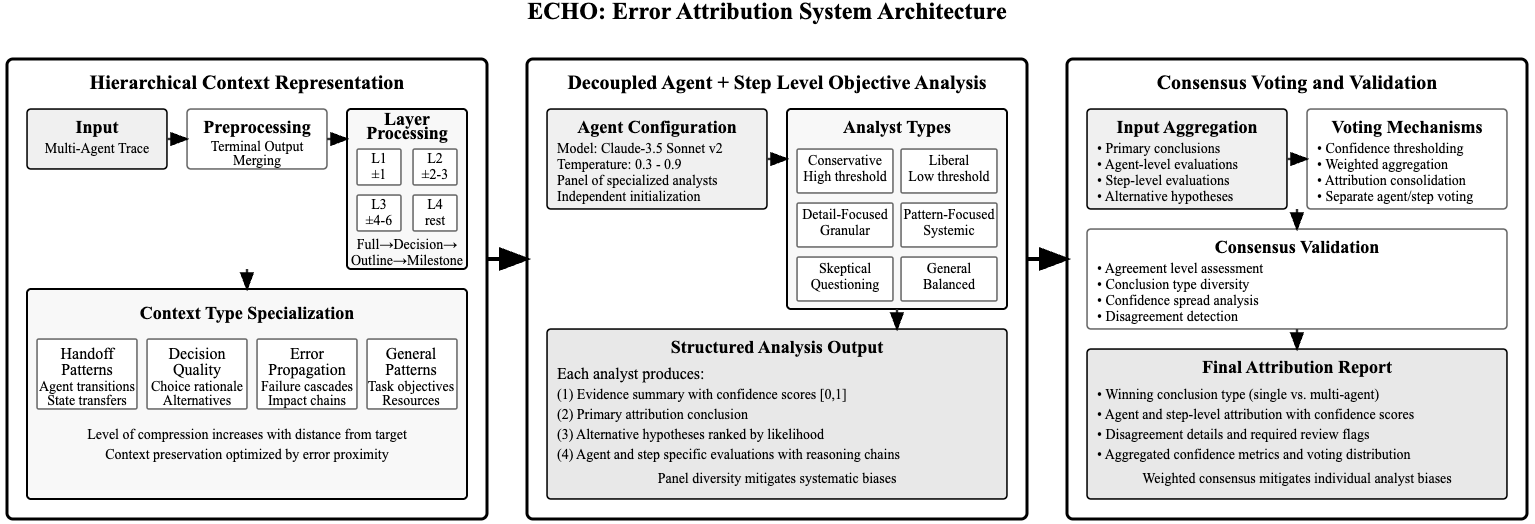
\includegraphics[width=\linewidth]{svgviewer-png-output_latest_2.png}
    \caption{Figure 1: ECHO Architecture. The system comprises: (1) Hierarchical Context - processes traces through 4 compression layers (L1-L4: full content → milestones) with specialized modules for handoffs, decisions, errors, and patterns; (2) Decoupled Analysis - uses 6 specialized agents (conservative to balanced) generating structured outputs with evidence, confidence scores, and hypotheses; (3) Consensus Voting - aggregates analyses via confidence-weighted voting and disagreement resolution.}
    \label{fig:figure_1}
\end{figure}
\subsection{Hierarchical Context Representation}

Error attribution in multi-agent systems faces a fundamental tension: while comprehensive context is crucial for accurate attribution, processing limitations make it impractical to analyze full interaction traces $\tau$ of $n$ agents with equal detail. Traditional approaches typically restrict analysis to immediate positional neighbors (±1 agent), presenting critical limitations. This narrow window fails to capture long-range dependencies where errors propagate across multiple steps and misses crucial context from causally relevant agents outside this window (e.g. error in initial problem formulation manifesting several steps later, or early incorrect assumptions propagating through multiple agents before causing a failure). ECHO addresses these limitations through a multi-layered hierarchical context representation ($C$) that captures both local and global interaction patterns.

% Approaches such as causal dependency graphs (that can trace information flow based on actual influence rather than temporal proximity) and semantic similarity methods (that can identify relevant agents regardless of their position in the trace) may be theoretically promising in mitigating these issues; however, they introduce prohibitive computational overhead and implementation complexity in real-world systems. ECHO instead leverages a pragmatic solution through a four-layer hierarchical context representation, inspired by human memory patterns where recent events are recalled in detail while distant events are stored as compressed summaries. This approach expands the context window to include the entire interaction trace while managing computational feasibility through strategic detail degradation at each layer.

% Hierarchical representation operates at 4 levels $L_1$ through $L_4$, as seen in Appendix \ref{appendix:echo_algorithm} and \ref{appendix:hierarchical_context}, to extract key information from agent / step interactions (via regex pattern matching). Its implementation employs specialized content extraction mechanisms for each layer $C_i$, as seen below:

Hierarchical representation operates at 4 levels $L_1$ through $L_4$, as seen in Appendix \ref{appendix:echo_algorithm} and \ref{appendix:hierarchical_context}, to extract key information from agent / step interactions (via regex pattern matching). While LLMs could potentially be used for more flexible content extraction, the computational overhead would be significant\textemdash a trade-off we explore further in Section 4.3. Its implementation employs specialized content extraction mechanisms for each layer $C_i$, as seen below: 

% \subsection{Hierarchical Context Representation}

% Error attribution in multi-agent systems faces a fundamental tension: while comprehensive context is crucial for accurate attribution, processing limitations make it impractical to analyze full interaction traces with equal detail. Traditional approaches typically restrict analysis to immediate temporal / positional neighbors (±1 agent), presenting critical limitations. This narrow window fails to capture long-range dependencies where errors propagate across multiple steps and misses crucial context from causally relevant agents outside this window. ECHO addresses these limitations through a multi-layered hierarchical context representation that captures both local and global interaction patterns.

% Approaches such as causal dependency graphs (that can trace information flow based on actual influence rather than temporal proximity) and semantic similarity methods (that can identify relevant agents regardless of their position in the trace) may be theoretically promising in mitigating these issues; however, they introduce prohibitive computational overhead and implementation complexity in real-world systems. ECHO instead leverages a pragmatic solution through a four-layer hierarchical context representation, inspired by human memory patterns where recent events are recalled in detail while distant events are stored as compressed summaries. This approach expands the context window to include the entire interaction trace while managing computational feasibility through strategic detail degradation at each layer.

% Our hierarchical representation operates at 4 levels to extract key information from agent / step interactions (via regex pattern matching). The implementation of this hierarchical representation employs specialized content extraction mechanisms for each layer, as seen below:

\begin{enumerate}
    \item \textbf{Immediate Context layer ($L_1$)}: Encompasses the target agent $i$ and its direct neighbors ($\tau_{i\pm1}$), preserving complete reasoning chains and interaction patterns. This layer maintains full agent content, including detailed decision-making processes, input-output relationships, and intermediate computations. This granular preservation enables precise analysis of local decision points and immediate error manifestations. Examples of these are: "Let me analyze the data... [Terminal Output]: DataFrame loaded, showing 500 rows". 
    \item \textbf{Local Context Layer ($L_2$)}: Spans $\tau_{i\pm2,3}$ steps from the target agent, focusing on tactical decision sequences and their interconnections. By preserving key reasoning chains while filtering routine operations, this layer reveals short-range error propagation patterns and local decision dependencies. This intermediate scope bridges the gap between immediate interactions and broader strategic patterns. Examples of these are focusing on specific patterns such as conclusive statements (e.g., "I conclude the optimal parameters are x=0.5, y=1.0") and logical transitions (e.g., "Therefore, we should use gradient descent"). 
    \item \textbf{Distant Context Layer ($L_3$)}: Covers $\tau_{i\pm4,5,6}$ steps through strategic compression, distilling agent interactions into concise outcome summaries. This layer captures essential state transitions, critical assumptions, and warning signals while filtering peripheral details. This compression enables identification of longer-range dependencies without overwhelming the analysis with excessive detail. Examples of these are critical state changes (e.g., "Model training failed: insufficient data"), error conditions (e.g., "Classification blocked: missing features"), and handoff information (e.g., "Received dataset with normalized features"). 
    \item \textbf{Global Context Layer ($L_4$)}: Encompasses the remaining interaction trace ($\tau_{remainder}$) through highly compressed milestone-based representation. By retaining only strategically significant decision points and major state transitions, this layer enables system-wide consistency checking and identification of broad error patterns. This high-level view ensures local decisions align with global objectives while maintaining computational feasibility. Examples of these include error propagation signals (e.g., "Persistent data quality errors"), major state transitions (e.g., "Switched from classification to regression"), and cross-agent dependencies (e.g., "Reusing parameters from Agent 2's optimization"). 
\end{enumerate}

This graduated extraction and compression approach adapts to different context types (handoff, decision quality, error propagation, general), enabling context-aware information preservation at each layer. Lastly, it is worth noting that when using regex-based extraction, real-world systems can be designed to generate reasoning traces with extractable keywords, effectively pre-seeding content for regex. This maintains efficiency while achieving accuracy comparable to more complex methods, making it practical for real applications.

% While this hierarchical representation remains position-based, its limitations have minimal practical impact on error attribution effectiveness. The primary theoretical drawback occurs in scenarios where temporally distant agents receive compressed representation despite their causal significance. However, our implementation mitigates this through three key mechanisms: (1) context-type aware pattern matching that preserves critical information even in compressed states, and (2) specialized extraction patterns for different types of agent interactions (handoff, decision-making, error conditions). This ensures that even at maximum compression, causally significant information is maintained through targeted pattern preservation, while still maintaining the computational efficiency of position-based processing.

\subsection{Objective Analysis}

% Traditional error attribution approaches often employ context-aware agents that are constrained to self-attribute blame, regardless of their actual contribution to the failure. This methodology introduces several critical limitations. First, it creates forced adversarial bias, where agents must generate attribution arguments even when their step was not erroneous, leading to artificial reasoning. Second, the absence of a null hypothesis mechanism prevents agents from legitimately concluding their non-involvement in the error. Third, these approaches suffer from confirmation bias due to their forced self-attribution nature, potentially overlooking more subtle or distributed error patterns. 

% ECHO implements a panel of $k$ objective analysis agents that evaluate the entire interaction trace $\tau$ through the hierarchical context representation $C$, as seen in the algorithm in Appendix \ref{appendix:echo_algorithm}. Rather than forcing self-attribution, each analysis agent independently examines all steps, providing attribution assessments with associated confidence scores $\sigma_j$. This approach allows for more nuanced attribution outcomes, including cases where no single agent is clearly responsible, multiple agents contributed through interaction effects, or where systemic issues span across multiple steps.
ECHO employs a panel of $k$ objective analysis agents that evaluate the full interaction trace $\tau$ through hierarchical context $C$ (algorithm in Appendix \ref{appendix:echo_algorithm}). Each analysis agent independently assesses all steps and provides confidence scores $\sigma_j$, enabling nuanced attributions that can identify distributed responsibility, interaction effects, and systemic issues spanning multiple agents or steps.

% The objective analysis framework integrates directly with the hierarchical context representation to facilitate multi-scale error attribution. Each analysis agent processes the four-layer context representation through a conversation summary that preserves critical indexing and context relationships. The agents examine potential errors at different granularities: analyzing detailed decision processes in $L_1$, evaluating intermediate state transitions in $L_2$, tracking error propagation patterns in $L_3$, and identifying systemic issues in $L_4$. To maintain analytical precision, the system explicitly requires agents to attribute errors only to steps where actual reasoning occurred. This structured approach enables attribution analysis across multiple context scales while maintaining precise step-level granularity.
The objective analysis framework leverages the hierarchical context through conversation summaries that preserve contextual relationships, enabling multi-scale error attribution. Agents examine errors across all layers: detailed decisions ($L_1$), state transitions ($L_2$), error propagation ($L_3$), and systemic issues ($L_4$). Furthermore, attribution is restricted to steps with explicit reasoning, ensuring precise analysis across context scales while maintaining step-level granularity.

The effectiveness of objective analysis depends critically on agent diversity to mitigate systematic biases. Rather than deploying identical agents that might propagate the same analytical biases, ECHO employs a panel of specialized analysts with roles $\rho_j$ (as seen in the code in Appendix \ref{appendix:objective_analysis}):
\begin{enumerate}
    \item \textbf{Conservative Analyst}: Requires strong, clear evidence for attribution, prefers single-agent attributions, maintains high confidence thresholds, and only attributes with definitive proof
    \item \textbf{Liberal Analyst}: Considers multi-agent error scenarios, identifies subtle error patterns, accepts moderate confidence thresholds, and makes attributions with reasonable evidence
    \item \textbf{Detail-Focused Analyst}: Examines specific evidence and exact wording, identifies subtle inconsistencies, focuses on fine-grained analysis, and prioritizes concrete evidence over patterns
    \item \textbf{Pattern-Focused Analyst}: Recognizes broader reasoning chains, tracks error propagation patterns, identifies recurring themes, and analyzes overall reasoning structure
    \item \textbf{Skeptical Analyst}: Questions underlying assumptions, explores alternative explanations, challenges conventional attributions, and examines validity of ground truth
    \item \textbf{General Analyst}: Maintains balanced perspective, considers all evidence types equally, focuses on obvious, impactful errors, and provides baseline objective evaluation
\end{enumerate}

% The implementation of each analysis agent is grounded in a structured evaluation framework. Each agent processes the conversation through a protocol that analyzes the conversation using both step-specific examination and hierarchical context relationships. The agents' analyses ($\epsilon_j$) are guided by specialized system prompts that reflect their assigned analytical focus. Each agent produces a structured output containing: (1) a summary of their investigation approach and findings, (2) detailed agent evaluations including error likelihood scores [0,1] and supporting evidence, (3) a primary conclusion specifying attribution type (single-agent or multi-agent), responsible agent(s), specific mistake step, and confidence score $\sigma_j$, and (4) alternative hypotheses that maintain reasonable likelihood. This structured approach ensures that even with varying analytical perspectives, the outputs maintain consistent format and comparable metrics for subsequent consensus voting.
Each analysis agent follows a structured evaluation protocol, examining both individual steps and their hierarchical context relationships. The agents' analyses ($\epsilon_j$) are guided by specialized prompts that reflect their assigned analytical focus, producing outputs with four components: (1) investigation summary, (2) detailed evaluations with error likelihood scores [0,1] and evidence, (3) primary conclusion specifying attribution type, responsible agent(s), mistake step, and confidence score $\sigma_j$, and (4) alternative hypotheses. This structure ensures consistent, comparable outputs for consensus voting across diverse analytical perspectives.

% This intentional diversity in analytical approaches - analogous to a review panel with different expertise - helps prevent echo-chamber effects in attribution. While our implementation achieves this diversity through role-specific prompts and temperatures, the framework supports other diversification mechanisms such as varying models, different LLM configurations, or alternative reasoning strategies. The key principle remains: systematic bias mitigation through deliberate analytical diversity.
This approach prevents echo-chamber effects in attribution through intentional perspective diversity. While this was implemented in ECHO through role-specific prompts and temperatures, the framework accommodates other diversification methods (different models, LLM configurations, or reasoning strategies)\textemdash all serving the core principle of bias mitigation through analytical diversity.


\subsection{Consensus Voting}
The final component of ECHO is a consensus voting mechanism that aggregates analyses from the panel of $k$ objective analysts, as seen in Appendix \ref{appendix:consensus_voting}. The voting system operates through weighted confidence consensus, where each analyst's attribution is weighted by their reported confidence level $\sigma_j$, subject to a minimum confidence threshold $\delta$ to filter out low-confidence attributions.

The consensus mechanism processes 3 key components from each analysis $A_t^j$ (where $t \in \{\text{agent}, \text{step}\}$): (1) Primary Conclusions\textemdash that considers core attribution decisions including the attribution type, responsible agent(s), and specific error step; (2) Agent Evaluations\textemdash that provides assessments of each agent's error likelihood and supporting evidence; and (3) Alternative Hypotheses\textemdash that considers secondary attribution possibilities that maintain reasonable likelihood.

The voting process follows a hierarchical decision structure, that first determines the winning conclusion type through weighted confidence aggregation of each analyzer's agent and step vote ($V_a, V_s$). Then for single/multi-agent conclusions, ECHO identifies specific agents through confidence-weighted attribution votes ($\omega_a$), after which it validates and aggregates step-level predictions ($\omega_s$). Finally it synthesizes supporting reasoning from the highest-confidence attributions.

The system explicitly handles disagreements through disagreement analysis $\phi$ by examining: (1) conclusion diversity (number of different conclusion types); (2) confidence spread across analysts ($\max(\sigma_j) - \min(\sigma_j)$); (3) attribution consistency between agent and step-level predictions; (4) need for additional review when high disagreement exists (spread > 0.5) or multiple conflicting high-confidence attributions emerge.

This structured voting approach ensures that the final attribution (ConsensusResult($\omega_a, \omega_s, \phi$)) reflects the collective analysis while maintaining sensitivity to strong minority opinions and potential edge cases. The combination of confidence weighting and explicit disagreement handling provides robustness against individual analyst biases while preserving valuable insights from dissenting views.

\section{Results and Analysis}
\subsection{Experimental Setup}

We evaluate our implementations using the Who\&When benchmark \cite{zhang2025agent}, a comprehensive dataset comprising failure logs from LLM-powered multi-agent systems. This benchmark is particularly suitable for error attribution evaluation as it provides fine-grained failure annotations across diverse scenarios, including both algorithm-generated and hand-crafted multi-agent interactions.

\textbf{Dataset Characteristics} - The benchmark consists of 2 distinct subsets: (1) Algorithm-Generated: systematic failure logs from automated multi-agent interactions; (2) Hand-Crafted: curated failure scenarios designed to capture complex error patterns. Each failure log is annotated with the failure-responsible agent; the specific step where the error occurred; and detailed failure reasoning.

\textbf{Evaluation Protocol} - We assess each implementation across 4 experimental conditions: (1) Algorithm-Generated with ground truth; (2) Algorithm-Generated without ground truth; (3) Hand-Crafted with ground truth; and (4) Hand-Crafted without ground truth. Attribution accuracy is measured at 2 levels: agent-level (referring to the correct identification of the failure-responsible agent; and step-level (referring to the correct identification of the specific error step).

% \textbf{Implementation Details} - Our framework employs Claude 3.5 Sonnet v2 as the base LLM, with varying temperatures between 0.3 and 0.9 across 3 randomly sampled different analysis agents to balance creativity and consistency. Other than that, the top-p employed is 0.9; and the maximum tokens is 4096.

% \textbf{Implementation Details} - Our framework employs Claude 3.5 Sonnet v2 as the base LLM, with varying temperatures between 0.3 and 0.9 across 3 randomly sampled different analysis agents (from a pool of 6 specialist types) to balance creativity and consistency. We use a minimum confidence threshold ($\delta = 0.3$) for filtering attributions in the consensus voting mechanism. The context layer parameters are fixed at L1: ±1, L2: ±2-3, L3: ±4-6, and L4 covering the remainder of the trace. Other hyperparameters include top-p of 0.9 and maximum tokens of 4096. Our implementation assumes position-based context importance, independence between analysis agents, and treats errors as primarily additive rather than emergent.

\textbf{Implementation Details} - Our framework employs Claude 3.5 Sonnet v2 as the base LLM, with varying temperatures between 0.3 and 0.9 across 3 randomly sampled analysis agents (from a pool of 6 specialists) for every scenario, to balance analytical diversity while reducing computational overhead. We use a confidence threshold ($\delta = 0.3$) for filtering attributions in the consensus voting mechanism, to balance inclusion of diverse perspectives while filtering out highly uncertain predictions. This implementation assumes position-based contextual importance, independence between analysis agents, and treats errors as primarily additive rather than emergent.
% Other hyperparameters include top-p of 0.9 and maximum tokens of 4096. 

\subsection{Comparative Analysis of Implementations}

We evaluate 4 progressive implementations of error attribution, each building upon the limitations of its predecessor:

\textbf{Implementation 1 (I1) - Fixed Context Window}:
Represents the baseline approach using a fixed context window (±1 step), where a context-aware agent analyzes each step with its immediate neighbors, followed by a final judge agent for attribution decisions.

\textbf{Implementation 2 (I2) - Hierarchical Context}:
Enhances I1 by replacing the fixed context window with a four-layer hierarchical context representation, maintaining the same attribution mechanism but providing graduated access to the full interaction trace.

\textbf{Implementation 3 (I3) - Objective Analysis}:
Builds upon I2's hierarchical context by replacing the context-aware agent and judge agent with a panel of specialized objective analyst agents and performing consensus voting on those outcomes, enabling diverse analytical perspectives.

\textbf{Implementation 4 (I4) - Decoupled Attribution}:
Refines I3 by separating the attribution process into two distinct phases: agent-level attribution to identify responsible agents, followed by step-level attribution to pinpoint specific error points, allowing for more focused analysis at each level.

\subsubsection{Performance of ECHO}

% \begin{table}[t]
% \caption{Performance of ECHO across different datasets and configurations}
% \label{tab:echo-results}
% \centering
% \small
% \begin{tabular}{lccccc}
% \toprule
% & \multicolumn{2}{c}{Hand-Crafted Dataset} & \multicolumn{2}{c}{Algorithm-Generated Dataset} & \\
% \cmidrule(lr){2-3} \cmidrule(lr){4-5}
% Metric & With GT & Without GT & With GT & Without GT & \\
% \midrule
% \multicolumn{5}{l}{\textbf{Agent-Level Accuracy}} & \\
% Random & 0.120 & 0.120 & 0.291 & 0.291 & \textit{fraction 0-1}\\
% All-at-Once & 0.552 & 0.534 & 0.543 & 0.511 & \textit{fraction 0-1}\\
% Step-by-Step & 0.345 & 0.328 & 0.352 & 0.260 & \textit{fraction 0-1}\\
% Binary Search & 0.517 & 0.362 & 0.441 & 0.301 & \textit{fraction 0-1} \\
% \midrule[\heavyrulewidth]
% \textbf{ECHO (ours)} & \textbf{0.684} & \textbf{0.679} & \textbf{0.688} & \textbf{0.672} & \textit{fraction 0-1}\\
% \midrule
% \multicolumn{5}{l}{\textbf{Step-Level Accuracy (Exact)}} & \\
% Random & 0.042 & 0.042 & 0.191 & 0.191 & \textit{fraction 0-1} \\
% All-at-Once & 0.053 & 0.035 & 0.125 & 0.135 & \textit{fraction 0-1}\\
% Step-by-Step & 0.070 & 0.088 & 0.255 & 0.153 & \textit{fraction 0-1}\\
% Binary Search & 0.069 & 0.069 & 0.240 & 0.166 & \textit{fraction 0-1}\\
% \midrule[\heavyrulewidth]
% \textbf{ECHO (ours)} & \textbf{0.281} & \textbf{0.268} & \textbf{0.272} & \textbf{0.288} & \textit{fraction 0-1}\\
% \midrule
% \multicolumn{6}{l}{\textbf{Step-Level with Tolerance}} \\
% \multicolumn{6}{l}{\textit{Hand-Crafted with GT:}} \\
% All-at-Once & 0.121 & -- & -- & -- & \textit{±1 step} \\
% & 0.198 & -- & -- & -- & \textit{±2 steps} \\
% & 0.302 & -- & -- & -- & \textit{±3 steps} \\
% & 0.371 & -- & -- & -- & \textit{±4 steps} \\
% & 0.431 & -- & -- & -- & \textit{±5 steps} \\
% Step-by-Step & 0.147 & -- & -- & -- & \textit{±1 step} \\
% & 0.164 & -- & -- & -- & \textit{±2 steps} \\
% & 0.181 & -- & -- & -- & \textit{±3 steps} \\
% & 0.319 & -- & -- & -- & \textit{±4 steps} \\
% & 0.336 & -- & -- & -- & \textit{±5 steps} \\
% Binary Search & 0.138 & -- & -- & -- & \textit{±1 step} \\
% & 0.190 & -- & -- & -- & \textit{±2 steps} \\
% & 0.224 & -- & -- & -- & \textit{±3 steps} \\
% & 0.319 & -- & -- & -- & \textit{±4 steps} \\
% & 0.362 & -- & -- & -- & \textit{±5 steps} \\
% \midrule[\heavyrulewidth]
% \textbf{ECHO (ours)} & \textbf{0.351} & \textbf{0.321} & \textbf{0.336} & \textbf{0.368} & \textit{±1 step} \\
% & \textbf{0.386} & \textbf{0.357} & \textbf{0.508} & \textbf{0.504} & \textit{±2 steps} \\
% & \textbf{0.421} & \textbf{0.393} & \textbf{0.572} & \textbf{0.552} & \textit{±3 steps} \\
% & \textbf{0.579} & \textbf{0.518} & \textbf{0.660} & \textbf{0.664} & \textit{±4 steps} \\
% & \textbf{0.614} & \textbf{0.607} & \textbf{0.704} & \textbf{0.712} & \textit{±5 steps} \\
% \midrule
% \multicolumn{6}{l}{\textbf{Computational Cost}} \\
% % \multicolumn{6}{l}{\textit{Hand-Crafted with GT:}} \\
% Binary Search & 34,659 & -- & -- & -- & \textit{tokens} \\
% All-at-Once & 17,106 & -- & -- & -- & \textit{tokens} \\
% Step-by-Step & 87,720 & -- & -- & -- & \textit{tokens} \\
% \midrule[\heavyrulewidth]
% \textbf{ECHO (ours)} & 53,701 & 52,136 & 19,156 & 19,297 & \textit{tokens} \\
% Avg. LLM Calls & 7 & 7 & 7 & 7 & \textit{invocations} \\
% Avg. Cost & 0.151 & 0.146 & 0.048 & 0.048 & \textit{(\$)}\\
% \bottomrule
% \end{tabular}
% \end{table}

% \begin{table}[t]
% \caption{Performance of ECHO across different datasets and configurations}
% \label{tab:echo-results}
% \centering
% \small
% \begin{tabular}{lcccc}
% \toprule
% & \multicolumn{2}{c}{Hand-Crafted Dataset} & \multicolumn{2}{c}{Algorithm-Generated Dataset} \\
% \cmidrule(lr){2-3} \cmidrule(lr){4-5}
% Metric & With GT & Without GT & With GT & Without GT \\
% \midrule
% \multicolumn{5}{l}{\textbf{Agent-Level Accuracy}} \\
% Random & 0.120 & 0.120 & 0.291 & 0.291 \\
% All-at-Once & 0.552 & 0.534 & 0.543 & 0.511 \\
% Step-by-Step & 0.345 & 0.328 & 0.352 & 0.260 \\
% Binary Search & 0.517 & 0.362 & 0.441 & 0.301 \\
% \midrule[\heavyrulewidth]
% \textbf{ECHO (ours)} & \textbf{0.684} & \textbf{0.679} & \textbf{0.688} & \textbf{0.672} \\
% \midrule
% \multicolumn{5}{l}{\textbf{Step-Level Accuracy (Exact)}} \\
% Random & 0.042 & 0.042 & 0.191 & 0.191 \\
% All-at-Once & 0.053 & 0.035 & 0.125 & 0.135 \\
% Step-by-Step & 0.070 & 0.088 & 0.255 & 0.153 \\
% Binary Search & 0.069 & 0.069 & 0.240 & 0.166 \\
% \midrule[\heavyrulewidth]
% \textbf{ECHO (ours)} & \textbf{0.281} & \textbf{0.268} & \textbf{0.288} & \textbf{0.272} \\
% \midrule
% \multicolumn{5}{l}{\textbf{Step-Level with Tolerance} \textit{(Hand-Crafted with GT)}} \\
% & All-at-Once & Step-by-Step & Binary Search & \textbf{ECHO (ours)} \\
% ±1 step & 0.121 & 0.147 & 0.138 & \textbf{0.351} \\
% ±2 steps & 0.198 & 0.164 & 0.190 & \textbf{0.386} \\
% ±3 steps & 0.302 & 0.181 & 0.224 & \textbf{0.421} \\
% ±4 steps & 0.371 & 0.319 & 0.319 & \textbf{0.579} \\
% ±5 steps & 0.431 & 0.336 & 0.362 & \textbf{0.614} \\
% \midrule
% \multicolumn{5}{l}{\textbf{Token Cost} \textit{(Hand-Crafted with GT)}} \\
% & All-at-Once & Step-by-Step & Binary Search & \textbf{ECHO (ours)} \\
% Tokens & \textbf{17,106} & 87,720 & 34,659 & 53,701 \\
% \bottomrule
% \end{tabular}
% \end{table}

\begin{table}[t]
\caption{Performance of ECHO across different datasets and configurations}
\label{tab:echo-results}
\centering
\small
\begin{tabular}{lccccc}
\toprule
& \multicolumn{2}{c}{Hand-Crafted Dataset} & \multicolumn{2}{c}{Algorithm-Generated Dataset} & \\
\cmidrule(lr){2-3} \cmidrule(lr){4-5}
Method & With GT & Without GT & With GT & Without GT & P-value$^{\dagger}$ \\
\midrule
\multicolumn{6}{l}{\textbf{Agent-Level Accuracy}} \\
Random & 0.120 & 0.120 & 0.291 & 0.291 & <0.001 \\
All-at-Once & 0.577 & 0.529 & 0.563 & 0.530 & 0.032 \\
Step-by-Step & 0.360 & 0.343 & 0.397 & 0.283 & <0.001 \\
Binary Search & 0.517 & 0.362 & 0.441 & 0.301 & 0.007 \\
\midrule[\heavyrulewidth]
\textbf{ECHO (ours)} & \textbf{0.684} & \textbf{0.679} & \textbf{0.688} & \textbf{0.672} & - \\
\midrule
\multicolumn{6}{l}{\textbf{Step-Level Accuracy (Exact)}} \\
Random & 0.042 & 0.042 & 0.191 & 0.191 & <0.001 \\
All-at-Once & 0.060 & 0.021 & 0.152 & 0.145 & <0.001 \\
Step-by-Step & 0.066 & 0.069 & 0.274 & 0.178 & 0.003 \\
Binary Search & 0.069 & 0.069 & 0.240 & 0.166 & 0.012 \\
\midrule[\heavyrulewidth]
\textbf{ECHO (ours)} & \textbf{0.281} & \textbf{0.268} & \textbf{0.288} & \textbf{0.272} & - \\
\midrule
\multicolumn{6}{l}{\textbf{Step-Level with Tolerance} \textit{(Hand-Crafted with GT)}} \\
& All-at-Once & Step-by-Step & Binary Search & \textbf{ECHO (ours)} & P-value$^{\dagger}$ \\
±1 step & 0.149 & 0.166 & 0.138 & \textbf{0.351} & <0.001 \\
±2 steps & 0.223 & 0.189 & 0.190 & \textbf{0.386} & 0.004 \\
±3 steps & 0.350 & 0.209 & 0.224 & \textbf{0.421} & 0.029 \\
±4 steps & 0.380 & 0.294 & 0.319 & \textbf{0.579} & 0.006 \\
±5 steps & 0.428 & 0.351 & 0.362 & \textbf{0.614} & 0.008 \\
\midrule
\multicolumn{6}{l}{\textbf{Token Cost} \textit{(Hand-Crafted with GT)}} \\
& All-at-Once & Step-by-Step & Binary Search & \textbf{ECHO (ours)} & - \\
Tokens & \textbf{17,106} & 87,720 & 34,659 & 53,701 & - \\
\bottomrule
\multicolumn{6}{l}{$^{\dagger}$P-values compare ECHO against each baseline using chi-squared test.} \\
\end{tabular}
\end{table}

%TODO: INCLUDE STAT SIG IN TABLES / DIAGRAMS / PLOTS DONE
%TODO: MAYBE DIVIDE TABLES
%TODO: MAYBE ANONYMOUS CODE REPO
%TODO: JUSTIFICATION OF HYPERPARAMETER CHOICES -- DONE
%TODO: ASSUMPTIONS -- DONE
ECHO demonstrates robust statistically significant performance (P < 0.05) across both hand-crafted and algorithm-generated datasets, with several notable patterns emerging from the results:

\textbf{Agent-Level Attribution}:
% The system achieves consistent agent-level accuracy ($\sim$68\%) across all configurations, with minimal degradation $\sim$1--2\% when ground truth is withheld. This suggests that ECHO's agent-level attribution mechanism is robust and doesn't heavily rely on ground truth information. The similar performance across both dataset types (hand-crafted: 68.4\%, algorithm-generated: 68.8\%) indicates good generalization across different interaction patterns.

The system achieves consistent agent-level accuracy ($\sim$68\%) across all configurations, with minimal degradation (1--2\%) when ground truth is withheld. Furthermore, the similar performance across both dataset types (hand-crafted: 68.4\%, algorithm-generated: 68.8\%) further demonstrates ECHO's robust generalization capabilities across different interaction patterns. This ground truth independence, combined with consistent cross-dataset performance, makes ECHO particularly valuable for deployment in dynamic, real-world AI systems where there is generally an absence of labeled data.

\textbf{Step-Level Attribution}:
% Exact step-level accuracy is notably lower ($\sim$27--28\%), reflecting the increased difficulty of precise step identification. However, when considering tolerance ranges, accuracy improves substantially:
% - With ±3 steps tolerance, accuracy reaches 42.1\% for hand-crafted and 57.2\% for algorithm-generated datasets
% - At ±5 steps tolerance, accuracy exceeds 60\% across all configurations
% - Algorithm-generated datasets show better tolerance scaling, reaching 70.4\% accuracy at ±5 steps
Although ECHO still outperforms prior methods with statistical significance, step-level precision still proves challenging, with exact matches at 27--28\%. However, accuracy improves significantly when accounting for step tolerance. With ±3 steps, accuracy reaches 42.1\% for hand-crafted dataset with ground truth; and when further extended to ±5 steps, accuracy reaches 61.4\%\textemdash again, maintaining superior performance over baselines.

\textbf{Impact of Ground Truth}:
The minimal difference in performance between configurations with and without ground truth (typically <2\% variation) suggests that ECHO's architecture effectively leverages interaction patterns and context for attribution, rather than relying on ground truth information. This is particularly important for real-world applications where ground truth may not be available.

\textbf{Token Counts}:
% ECHO maintains consistent computational patterns across configurations and significantly lowers token usage for algorithm-generated datasets (~19K vs $\sim$54K tokens), ensuring cost-effective processing (\$0.048 for algorithm-generated, \$0.15 for hand-crafted cases).
ECHO demonstrates moderate token efficiency, using $\sim$54K tokens compared to $\sim$88K for Step-by-Step and $\sim$17K for All-at-Once approaches on hand-crafted datasets. While higher than the simplest baseline, ECHO's token usage reflects its balanced approach to comprehensive analysis, maintaining reasonable processing costs of \$0.15 per example with Claude 3.5 Sonnet v2.

The results demonstrate ECHO's capability to provide reliable agent-level attribution while offering flexible step-level identification with tolerance ranges. The system's consistent performance across different datasets and configurations, combined with its reasonable computational overhead, makes it suitable for practical applications in error attribution for multi-agent systems.

\subsection{Impact of ECHO Components Via Ablation}

% \begin{table}[t]
% \caption{Ablation Study: Impact of Decoupled Analysis}
% \label{tab:ablation-decoupled}
% \centering
% \small
% \begin{tabular}{lcccc}
% \toprule
% & \multicolumn{2}{c}{Hand-Crafted Dataset} & \multicolumn{2}{c}{Algorithm-Generated Dataset} \\
% \cmidrule(lr){2-3} \cmidrule(lr){4-5}
% Metric & With GT & Without GT & With GT & Without GT \\
% \midrule
% \multicolumn{5}{l}{\textbf{Agent-Level Accuracy}} \\
% Unified (I3) & 0.610 & 0.589 & 0.651 & 0.635 \\
% Decoupled (I4) & \textbf{0.684} & \textbf{0.679} & \textbf{0.688} & \textbf{0.672} \\
% \midrule
% \multicolumn{5}{l}{\textbf{Step-Level Accuracy}} \\
% Unified (I3) & 0.232 & 0.232 & \textbf{0.444} & \textbf{0.461} \\
% Decoupled (I4) & \textbf{0.281} & \textbf{0.268} & 0.272 & 0.288 \\
% \midrule
% \multicolumn{5}{l}{\textbf{Computational Efficiency}} \\
% \multicolumn{5}{l}{\textit{Average Tokens per Item:}} \\
% Unified (I3) & 67.5K & 66.5K & 12.5K & 12.6K \\
% Decoupled (I4) & \textbf{33.0K}$^*$ & \textbf{32.5K}$^*$ & \textbf{12.7K}$^*$ & \textbf{12.7K}$^*$ \\
% \midrule
% \multicolumn{5}{l}{\textit{Average LLM Calls:}} \\
% Unified (I3) & \textbf{4.0} & \textbf{4.0} & \textbf{4.0} & \textbf{4.0} \\
% Decoupled (I4) & 7.0 & 7.0 & 7.0 & 7.0 \\
% \bottomrule
% \multicolumn{5}{l}{\small $^*$Sum of agent-level and step-level analysis tokens} \\
% \end{tabular}
% \end{table}

\begin{table}[t]
\caption{Ablation Study: Impact of Each Component}
\label{tab:ablation-combined}
\centering
\small
\begin{tabular}{lccccc}
\toprule
& \multicolumn{2}{c}{Hand-Crafted Dataset} & \multicolumn{2}{c}{Algorithm-Generated Dataset} & \\
\cmidrule(lr){2-3} \cmidrule(lr){4-5}
Implementation & With GT & Without GT & With GT & Without GT & P-value$^{\ddagger}$ \\
\midrule
\multicolumn{6}{l}{\textbf{Agent-Level Accuracy}} \\
Fixed Context (I1)$^{\dagger}$ & 0.286 & 0.265 & 0.461 & 0.452 & - \\
+ Hierarchical (I2)$^{\dagger}$ & 0.447 & 0.429 & 0.523 & 0.508 & 0.037 \\
+ Objective Analysis (I3) & 0.610 & 0.589 & 0.651 & 0.635 & 0.043 \\
+ Decoupled Attribution (I4) & \textbf{0.684} & \textbf{0.679} & \textbf{0.688} & \textbf{0.672} & 0.196 \\
\midrule
\multicolumn{6}{l}{\textbf{Step-Level Accuracy}} \\
Fixed Context (I1)$^{\dagger}$ & 0.151 & 0.143 & 0.157 & 0.140 & - \\
+ Hierarchical (I2)$^{\dagger}$ & 0.170 & 0.166 & 0.192 & 0.175 & 0.398 \\
+ Objective Analysis (I3) & 0.232 & 0.218 & \textbf{0.461} & \textbf{0.444} & <0.001 \\
+ Decoupled Attribution (I4) & \textbf{0.281} & \textbf{0.268} & 0.288 & 0.272 & 0.211 \\
\midrule
\multicolumn{6}{l}{\textbf{Token Cost}} \\
Fixed Context (I1)$^{\dagger}$ & 4.02M & 3.93M & 319K & 317K & - \\
+ Hierarchical (I2)$^{\dagger}$ & 7.70M & 7.66M & 407K & 405K & - \\
+ Objective Analysis (I3) & 67.5K & 66.5K & \textbf{12.6K} & \textbf{12.5K} & - \\
+ Decoupled Attribution (I4) & \textbf{33.0K} & \textbf{32.5K} & 12.8K & 12.7K & - \\
\bottomrule
\multicolumn{6}{l}{\small $^{\dagger}$Hand-Crafted Dataset results for I1 and I2 based on limited sample of shorter traces} \\
\multicolumn{6}{l}{\small $^{\ddagger}$P-values compare each component with previous implementation} \\
\end{tabular}
\end{table}

\textbf{The Question of Unifying or Decoupling Objective Analyses}

% The effectiveness of decoupling agent-level and step-level analyses shows a striking dependency on trace length (Table \ref{tab:ablation-combined}). For shorter algorithm-generated traces, unified analysis achieves strong performance (65.1\% agent-level, 44.4\% step-level accuracy), with decoupling actually harming step-level prediction despite marginal agent-level improvements. However, this dynamic reverses for longer hand-crafted traces, where decoupling improves both agent-level accuracy (61.0\% to 68.4\%) and step-level prediction consistency while significantly reducing token usage (67K to ~17K tokens per task). This reveals a key insight: while shorter traces benefit from unified analysis maintaining complete contextual information within the LLM's comfortable processing range, longer traces approaching model limits benefit from the complexity management offered by decoupled analysis.


% The relationship between context length and attribution performance reveals interesting insights about when to unify or decouple agent-level and step-level analyses (Table \ref{tab:ablation-combined}). For shorter traces in the algorithm-generated dataset, unified objective analysis achieves strong performance with 65.1\% agent-level accuracy and notably high step-level accuracy (46.1\% exact). While decoupling marginally improves agent-level accuracy to 68.8\%, it significantly deteriorates step-level prediction to 28.8\%, albeit not statistically significant at P < 0.05. This counter-intuitive result suggests that reducing contextual burden through task separation can be detrimental when working within the LLM's comfortable processing range (~13K tokens for unified analysis vs. 6K/7K tokens for decoupled components).

The analysis of context length reveals key insights about unified versus decoupled attribution (Table \ref{tab:ablation-combined}). For shorter algorithm-generated traces, unified analysis achieves strong results (65.1\% agent-level, 46.1\% step-level accuracy), while decoupling shows mixed effects: marginal improvement in agent-level accuracy (68.8\%) but notable decline in step-level precision (28.8\%). This suggests that splitting attribution tasks can be counterproductive when operating within the LLM's comfortable processing range ($\sim$13K tokens unified vs. $\sim$6K+7K tokens decoupled).

% The situation reverses for longer traces in the hand-crafted dataset, where unified analysis struggles with step-level prediction (23.2\% exact) while maintaining moderate agent-level accuracy (61.0\%). Switching to decoupled analysis improves agent-level accuracy to 68.4\% and provides more consistent step-level prediction patterns with an accuracy of 28.1\%, coinciding with significant token reduction per task (from ~67K tokens for unified analysis to ~13K/19K tokens for decoupled components). These findings indicate that the effectiveness of decoupled attribution is context-length dependent: shorter traces benefit from unified analysis maintaining complete contextual information, while longer traces approaching model limits benefit from the complexity management of decoupled analysis.

For longer hand-crafted traces, unified analysis struggles with step-level precision (23.2\%) while maintaining moderate agent-level accuracy (61.0\%). Decoupling improves performance (68.4\% agent-level, 28.1\% step-level) while significantly reducing per-task tokens (from $\sim$67K to $\sim$13K+19K). This reveals context-length dependency: shorter traces benefit from unified analysis's complete context, while longer traces near model limits favor decoupled analysis' complexity management.

\textbf{The Computational Overhead Resolution By Using Objective Analysis}

% The introduction of objective analysis (I3) demonstrates the limitations of using context-aware agents for error attribution, even when provided with comprehensive context. While both fixed context (I1) and hierarchical context (I2) implementations use context-aware agents that examine trace information, this approach proves computationally intensive due to the need for repeated agent analysis of the same information. The shift to objective analysis significantly improves efficiency, reducing average token usage by two orders of magnitude for hand-crafted datasets (from millions to thousands of tokens) and by a factor of 20 for algorithm-generated datasets. This is reflected in the dramatic reduction of LLM calls (from ~20 to 4 calls), while simultaneously improving attribution accuracy by 16.3\% for agent-level and 6.2\% for step-level attribution with statistical significance (P < 0.05), as seen in Table \ref{tab:ablation-combined}. These results suggest that moving away from context-aware agents toward objective analysis is crucial for practical deployment, as it maintains the benefits of comprehensive context while enabling efficient processing of longer traces through more sophisticated analytical approaches.
The shift to objective analysis (I3) reveals key limitations of context-aware agents in error attribution. While fixed (I1) and hierarchical (I2) context implementations leverage trace information, their repeated analysis proves computationally intensive. Objective analysis dramatically improves efficiency, reducing token usage by 60-110x for hand-crafted cases, and by 25-30x for algorithm-generated cases, while still improving accuracy ($\sim$+16.3\% agent-level and $\sim$+6.2\% step-level at P < 0.05) as shown in Table \ref{tab:ablation-combined}. These results demonstrate that objective analysis is crucial for practical deployment, enabling efficient processing of longer traces while maintaining comprehensive context benefits.\newline

\textbf{Switching from Fixed-Window Context to Hierarchical Context}

% The benefits of hierarchical context representation over fixed context windows are evident, even within the context-aware agent framework. Moving from fixed ±1 step context (I1) to hierarchical context (I2) improves agent-level accuracy by 16.1\% (statistically significant at P < 0.05) and step-level accuracy by 1.9\% (not statistically significant at P < 0.05) on hand-crafted data with ground truth, as seen in Table \ref{tab:ablation-combined}. This improvement demonstrates the value of graduated context preservation, where information detail decreases with distance from the target step. However, it's important to note that both I1 and I2 results for hand-crafted data are based on a subset of shorter traces, as the computational requirements for longer traces (50+ agents) proved prohibitive with context-aware agents. Despite this limitation to shorter traces, the consistent improvement in attribution accuracy suggests that hierarchical context representation provides valuable information for error attribution, a benefit that is later fully realized when combined with objective analysis. 
Hierarchical context shows clear advantages over fixed context windows within the context-aware framework. Shifting from fixed ±1 step (I1) to hierarchical context (I2) yields significant improvements in hand-crafted datasets: +16.1\% in agent-level accuracy (P < 0.05) and +1.9\% in step-level accuracy (not significant), as shown in Table \ref{tab:ablation-combined}. A similar trend is exhibited for the algorithm-generated dataset, with a +6.2\% in agent-level accuracy and +3.8\% in step-level accuracy.  This validates graduated context preservation, where detail decreases with distance from target steps. While analysis for the hand-crafted dataset was limited to shorter traces due to computational constraints with context-aware agents, the consistent accuracy improvements highlight hierarchical context's value\textemdash a benefit fully realized when combined with objective analysis.

\begin{table}[t]
\caption{Additional Ablations on Hand-Crafted Dataset with Ground Truth}
\label{tab:ablation-additional}
\centering
\small
\begin{tabular}{lcccc}
\toprule
Implementation & Agent-Level & Step-Level & Token Cost & P-value$^{\ddagger}$ \\
\midrule
\multicolumn{5}{l}{\textbf{LLM Capability}} \\
Claude-3 Haiku & 0.618 & 0.164 & 60,008 & 0.042 \\
\textbf{ECHO (Claude-3.5 Sonnet)} & 0.684 & \textbf{0.281} & \textbf{53,701} & - \\
Claude-3.7 Sonnet & \textbf{0.788} & 0.269 & 57,223 & 0.036 \\
\midrule
\multicolumn{5}{l}{\textbf{Hierarchical Context Method}} \\
\textbf{ECHO (Regex-based)} & 0.684 & 0.281 & \textbf{53,701} & - \\
LLM-based$^{\dagger}$ & \textbf{0.750} & \textbf{0.438} & 165,932 & - \\
\midrule
\multicolumn{5}{l}{\textbf{Objective Analyst Panel Size}} \\
\textbf{ECHO (3 Analysts)} & \textbf{0.684} & \textbf{0.281} & \textbf{53,701} & - \\
6 Analysts & 0.667 & 0.259 & 87,603 & 0.483 \\
\bottomrule
\multicolumn{5}{l}{\small $^{\dagger}$Tested on limited sample of shorter traces due to computational constraints} \\
\multicolumn{5}{l}{\small $^{\ddagger}$P-values compare with ECHO baseline for each sections} \\
\end{tabular}
\end{table}

% The introduction of objective analysis (I3) demonstrates substantial improvements over hierarchical context alone (I2) across all metrics (Table \ref{tab:ablation-combined}). For agent-level attribution, objective analysis improves accuracy by 18.1\%  on algorithm-generated data and 14.3\% on hand-crafted data, with ground truth. Step-level attribution shows even more dramatic improvements, particularly on algorithm-generated data where accuracy increases by 31.9\%.

% Most notably, objective analysis achieves these improvements while dramatically reducing computational overhead. The approach reduces average token usage by two orders of magnitude for hand-crafted datasets (7.66M to 88K tokens) and by a factor of 20 for algorithm-generated datasets (407K to 20K tokens). This efficiency gain is further reflected in the reduced number of LLM calls required per analysis (21.8 to 4.0 for hand-crafted, 9.7 to 4.0 for algorithm-generated).

% Two important caveats warrant discussion. First, while I2 implements hierarchical context extraction, it pairs this with a context-aware agent that examines the entire trace (rather than just immediate neighbors) to match the comprehensive context provided. This approach, while theoretically sound, becomes prohibitively expensive for longer traces. Second, the I2 results for hand-crafted data are based only on a subset of shorter traces, as the computational requirements for longer traces on the hand-crafted dataset (50+ agents) proved impractical. Even with this favorable bias toward shorter traces, I2's performance was substantially lower than I3, suggesting that its real-world performance on full-length traces would likely be even worse. This limitation is particularly evident in the token usage. and emphasizes why the efficiency gains achieved through objective analysis are crucial for practical deployment.

% \textbf{Our Commentary on the Who\&When Benchmark}

% While the Who\&When benchmark represents a significant step forward in evaluating error attribution systems, our experience with it suggests several opportunities for enhancement to better reflect real-world multi-agent system complexities. First, the benchmark would benefit from standardized categorization of problem types (numerical, coding, reasoning), enabling more granular analysis of algorithm effectiveness across different cognitive tasks. 

% More fundamentally, the benchmark could be extended to capture more complex architectural patterns. Current examples, while including basic orchestrator-subagent relationships, primarily follow sequential execution paths. Real-world systems often employ more sophisticated patterns such as parallel processing, hybrid parallel-sequential execution, and complex inter-agent dependencies. This limitation particularly affects the evaluation of error propagation detection in more nuanced scenarios. Additionally, the benchmark's assumption of single point failures doesn't fully represent real-world scenarios where multiple failure points may exist, or where initial errors might be amplified, mitigated, or transformed by subsequent agent actions.

% Lastly, the benchmark could be enhanced by incorporating systemic external errors that aren't attributable to specific agent reasoning steps. Examples include LLM provisioning issues, token limitations, or prompt engineering constraints - factors that can significantly impact system performance but operate outside individual agent decision processes. While the current benchmark provides a robust foundation for evaluating error attribution systems, these enhancements would better align it with the complexities and challenges encountered in production multi-agent systems.

% \section{Future Work}

% Building on ECHO's foundation, several promising research directions emerge. Future work could explore relevance-based architectures that dynamically adjust context preservation based on semantic relationships and causal dependencies, moving beyond position-based representation to better capture long-range interactions. The consensus mechanism could be enhanced through multi-agent debate protocols, enabling analysis agents to challenge each other's reasoning and request clarification, potentially leading to more robust attribution through structured analytical discourse. Additionally, developing methods for identifying and attributing emergent error patterns from step interactions, rather than treating them as additive effects, represents an important area for investigation. The attribution framework itself could evolve beyond binary assessment to incorporate error severity metrics and partial correctness evaluation, while the Who\&When benchmark could be enhanced with standardized problem-type categorization, complex architectural patterns, and examples with multiple or cascading failure points to better reflect real-world scenarios.

% While ECHO demonstrates the potential of combining hierarchical context representation, objective analysis, and consensus voting for error attribution, several limitations warrant discussion and suggest future research directions. First, our hierarchical context representation remains fundamentally position-based rather than relevance-based, potentially leading to suboptimal context preservation when causally significant interactions occur between distant steps. Future work could explore architectures that dynamically adjust context preservation based on semantic relationships and causal dependencies, complemented by more sophisticated compression mechanisms that preserve information based on predicted significance.

% The consensus voting mechanism currently lacks sophisticated cross-validation of competing attributions and multi-agent debate capabilities. Implementing debate protocols that allow analysis agents to challenge each other's reasoning and request clarification could lead to more robust attribution through structured analytical discourse. Additionally, our treatment of multi-step errors assumes additive rather than emergent effects, suggesting the need for methods that better identify and attribute complex error patterns arising from step interactions.

% A significant limitation lies in our binary approach to attribution correctness, where real-world errors often exist on a spectrum of severity and impact. Future work should move beyond binary attribution to incorporate error severity assessment and partial correctness evaluation, including metrics for error impact quantification. The Who\&When benchmark itself could be enhanced to better reflect real-world scenarios by incorporating standardized problem-type categorization, complex architectural patterns, and examples with multiple or cascading failure points.

\textbf{Additional Ablation Studies}

% We conducted several additional ablation studies on the hand-crafted dataset with ground truth to explore various aspects of ECHO's design. Model capability comparison between Claude-3 Haiku and Claude-3.7 Sonnet showed that stronger reasoning models improve performance at a statistically significant manner at P < 0.05 (61.8\% to 78.8\% agent-level accuracy, 16.4\% to 26.9\% step-level accuracy), while maintaining similar token usage (~60K tokens). Replacing regex-based hierarchical context extraction with LLM-based extraction on shorter traces showed promising results (75.0\% agent-level, 43.8\% step-level accuracy) but at substantial computational cost (165K vs. 54K tokens per item, with context extraction alone consuming 145K tokens) - making it computationally intractable for production systems with longer traces where token counts would scale prohibitively. Investigation of analyst panel size revealed that using all 6 analysts versus the default 3 showed minimal / not statistically significant performance difference (66.7\% vs. 68.4\% agent-level accuracy) while nearly doubling token usage (88K vs. 54K tokens), suggesting our default configuration effectively balances analytical diversity and computational efficiency. These results have been shown in Table \ref{tab:ablation-additional}.
Additional ablation studies on the hand-crafted dataset with ground truth reveal key design insights. Using stronger reasoning models significantly improve performance (P < 0.05): Claude-3.7 Sonnet achieves 78.8\% agent-level and 26.9\% step-level accuracy versus Haiku's 61.8\% and 16.4\%, maintaining similar token usage ($\sim$60K). Switching from regex-based context extraction to LLM-based context extraction shows promise (75.0\% agent-level, 43.8\% step-level) but proves computationally intractable ($\sim$166K vs. 54K tokens, with extraction alone using $\sim$145K). Lastly, expanding the analyst panel size from 3 to 6 yields minimal gains (68.4\% vs. 66.7\% agent-level) while doubling token usage (88K vs. 54K), validating our default configuration's efficiency. These results have been shown in Table \ref{tab:ablation-additional}.

\section{Conclusion}

% We introduce ECHO, a novel approach to error attribution in multi-agent systems that combines hierarchical context representation, decoupled objective analysis, and confidence-weighted consensus voting to address key challenges in analyzing complex interaction traces. Our results demonstrate substantial improvements over existing methods, particularly in handling longer traces where traditional approaches become computationally prohibitive. Building on these foundations, future research directions include developing relevance-based architectures for dynamic context preservation, enhancing the consensus mechanism through multi-agent debate protocols, and evolving the attribution framework to incorporate error severity metrics and partial correctness evaluation. Additionally, the Who\&When benchmark could be expanded with standardized problem-type categorization and complex architectural patterns to better reflect real-world scenarios. As multi-agent systems become increasingly prevalent, ECHO's efficient context representation and bias mitigation approach provides a promising foundation for debugging and maintaining these complex systems effectively.
We introduce ECHO, a novel approach to error attribution in multi-agent systems that combines hierarchical context representation, decoupled objective analysis, and confidence-weighted consensus voting. Our results demonstrate substantial improvements over existing baseline methods, particularly for longer traces where traditional approaches become prohibitive. Beyond immediate applications, ECHO's precise error attribution capabilities have broader implications for AI development: in reinforcement learning, it can help identify and eliminate false steps that may reduce model efficacy, while in single-agent optimization, it enables targeted prompt refinement for systems like GEPA \cite{agrawal2025gepareflectivepromptevolution} and DEEVO \cite{nair2025tournamentpromptsevolvingllm}. Future directions include developing relevance-based architectures for dynamic context preservation, enhancing the consensus mechanism through multi-agent debate protocols \cite{nair2025tournamentpromptsevolvingllm}, and incorporating error severity metrics as well as partial correctness evaluation. Additionally, the Who\&When benchmark could be expanded with standardized problem-type categorization and complex architectural patterns to better reflect real-world scenarios. As multi-agent systems proliferate, ECHO's efficient context handling and bias mitigation approach provides a crucial foundation for both debugging current systems and advancing AI development practices.

% This paper introduces ECHO, a novel approach to error attribution in multi-agent systems that addresses key challenges in analyzing complex interaction traces. By combining hierarchical context representation, decoupled objective analysis, and confidence-weighted consensus voting, ECHO demonstrates significant improvements over existing methods across both algorithm-generated and hand-crafted datasets. The hierarchical context representation enables comprehensive trace analysis while maintaining computational feasibility, while the panel of specialized analysts with diverse perspectives helps mitigate individual analytical biases. The decoupled attribution approach shows particular promise in handling longer, more complex traces where traditional methods become computationally prohibitive.

% Our results demonstrate substantial improvements in both agent-level and step-level attribution accuracy compared to baselines, while maintaining reasonable computational overhead. The system's performance remains robust even without ground truth information, suggesting its viability for real-world applications. While limitations exist in our current implementation, ECHO establishes a foundation for more sophisticated error attribution systems. As multi-agent systems become increasingly prevalent, robust error attribution mechanisms like ECHO will be crucial for debugging, improving, and maintaining these systems effectively.





% \section{Limitations}

% While ECHO demonstrates the potential of combining hierarchical context representation, objective analysis, and consensus voting for error attribution, several limitations warrant discussion. First, our hierarchical context representation, while effective, remains fundamentally position-based rather than relevance-based. This can lead to suboptimal context preservation when causally significant interactions occur between distant steps. Additionally, the current compression mechanism, though graduated, may still result in information loss that affects attribution accuracy.

% The consensus voting mechanism, while providing a structured approach to aggregating multiple perspectives, currently lacks sophisticated cross-validation of competing attributions. The absence of multi-agent debate or clarification mechanisms means that potentially valuable analytical discourse is lost. Furthermore, our treatment of multi-step errors assumes additive rather than emergent effects, potentially oversimplifying complex error patterns that arise from step interactions rather than individual step failures.

% A significant limitation lies in our binary approach to attribution correctness. Real-world errors often exist on a spectrum of severity and impact, which our current method doesn't capture. This simplification, while practical for initial implementation, may not fully represent the nuanced nature of errors in complex multi-agent systems.

% \section{Conclusion}

% This paper introduces ECHO, a novel approach to error attribution in multi-agent systems that addresses key challenges in analyzing complex interaction traces. By combining hierarchical context representation, decoupled objective analysis, and confidence-weighted consensus voting, ECHO demonstrates significant improvements over existing methods across both algorithm-generated and hand-crafted datasets. The hierarchical context representation enables comprehensive trace analysis while maintaining computational feasibility, while the panel of specialized analysts with diverse perspectives helps mitigate individual analytical biases. The decoupled attribution approach shows particular promise in handling longer, more complex traces where traditional methods become computationally prohibitive.

% Our results demonstrate that ECHO achieves substantial improvements in both agent-level and step-level attribution accuracy compared to baseline approaches, while maintaining reasonable computational overhead. The system's performance remains robust even without ground truth information, suggesting its viability for real-world applications where such information may be unavailable. Furthermore, our analysis of the Who\&When benchmark provides valuable insights for the future development of error attribution evaluation frameworks.

% While limitations exist in our current implementation, particularly around position-based context representation and binary attribution assessment, ECHO establishes a foundation for more sophisticated error attribution systems. Future work in developing relevance-based architectures, implementing multi-agent debate protocols, and incorporating error severity assessment could further advance the field. As multi-agent systems become increasingly prevalent in real-world applications, robust error attribution mechanisms like ECHO will be crucial for debugging, improving, and maintaining these systems effectively.


% \section{Future Work}

% Several promising directions emerge from these limitations and our experience with the Who\&When benchmark. For context representation, future work could explore relevance-based architectures that dynamically adjust context preservation based on semantic relationships and causal dependencies rather than positional proximity. This could be complemented by more sophisticated compression mechanisms that preserve information based on its predicted significance to error attribution.

% The consensus mechanism could be enhanced through implementation of multi-agent debate protocols, allowing analysis agents to challenge each other's reasoning and request clarification. This could lead to more robust attribution through structured analytical discourse. Additionally, developing methods for identifying and attributing emergent errors from step interactions, rather than treating them as collections of individual step failures, represents an important area for investigation.

% Future iterations should also move beyond binary attribution to incorporate error severity assessment and partial correctness evaluation. This could include developing metrics for error impact quantification and frameworks for understanding error propagation effects. The benchmark itself could be enhanced to better reflect real-world scenarios by incorporating standardized problem-type categorization, complex architectural patterns such as parallel and hybrid execution flows, and examples with multiple or cascading failure points. These enhancements, combined with the inclusion of systemic external errors and varying degrees of error severity, would enable more rigorous evaluation of attribution methods and drive the development of more robust algorithms.













% \subsection{Headings: second level}


% Second-level headings should be in 10-point type.


% \subsubsection{Headings: third level}


% Third-level headings should be in 10-point type.


% \paragraph{Paragraphs}


% There is also a \verb+\paragraph+ command available, which sets the heading in
% bold, flush left, and inline with the text, with the heading followed by 1\,em
% of space.


% \section{Citations, figures, tables, references}
% \label{others}


% These instructions apply to everyone.


% \subsection{Citations within the text}


% The \verb+natbib+ package will be loaded for you by default.  Citations may be
% author/year or numeric, as long as you maintain internal consistency.  As to the
% format of the references themselves, any style is acceptable as long as it is
% used consistently.


% The documentation for \verb+natbib+ may be found at
% \begin{center}
%   \url{http://mirrors.ctan.org/macros/latex/contrib/natbib/natnotes.pdf}
% \end{center}
% Of note is the command \verb+\citet+, which produces citations appropriate for
% use in inline text.  For example,
% \begin{verbatim}
%    \citet{hasselmo} investigated\dots
% \end{verbatim}
% produces
% \begin{quote}
%   Hasselmo, et al.\ (1995) investigated\dots
% \end{quote}


% If you wish to load the \verb+natbib+ package with options, you may add the
% following before loading the \verb+neurips_2024+ package:
% \begin{verbatim}
%    \PassOptionsToPackage{options}{natbib}
% \end{verbatim}


% If \verb+natbib+ clashes with another package you load, you can add the optional
% argument \verb+nonatbib+ when loading the style file:
% \begin{verbatim}
%    \usepackage[nonatbib]{neurips_2024}
% \end{verbatim}


% As submission is double blind, refer to your own published work in the third
% person. That is, use ``In the previous work of Jones et al.\ [4],'' not ``In our
% previous work [4].'' If you cite your other papers that are not widely available
% (e.g., a journal paper under review), use anonymous author names in the
% citation, e.g., an author of the form ``A.\ Anonymous'' and include a copy of the anonymized paper in the supplementary material.


% \subsection{Footnotes}


% Footnotes should be used sparingly.  If you do require a footnote, indicate
% footnotes with a number\footnote{Sample of the first footnote.} in the
% text. Place the footnotes at the bottom of the page on which they appear.
% Precede the footnote with a horizontal rule of 2~inches (12~picas).


% Note that footnotes are properly typeset \emph{after} punctuation
% marks.\footnote{As in this example.}


% \subsection{Figures}


% \begin{figure}
%   \centering
%   \fbox{\rule[-.5cm]{0cm}{4cm} \rule[-.5cm]{4cm}{0cm}}
%   \caption{Sample figure caption.}
% \end{figure}


% All artwork must be neat, clean, and legible. Lines should be dark enough for
% purposes of reproduction. The figure number and caption always appear after the
% figure. Place one line space before the figure caption and one line space after
% the figure. The figure caption should be lower case (except for first word and
% proper nouns); figures are numbered consecutively.


% You may use color figures.  However, it is best for the figure captions and the
% paper body to be legible if the paper is printed in either black/white or in
% color.


% \subsection{Tables}


% All tables must be centered, neat, clean and legible.  The table number and
% title always appear before the table.  See Table~\ref{sample-table}.


% Place one line space before the table title, one line space after the
% table title, and one line space after the table. The table title must
% be lower case (except for first word and proper nouns); tables are
% numbered consecutively.


% Note that publication-quality tables \emph{do not contain vertical rules.} We
% strongly suggest the use of the \verb+booktabs+ package, which allows for
% typesetting high-quality, professional tables:
% \begin{center}
%   \url{https://www.ctan.org/pkg/booktabs}
% \end{center}
% This package was used to typeset Table~\ref{sample-table}.


% \begin{table}
%   \caption{Sample table title}
%   \label{sample-table}
%   \centering
%   \begin{tabular}{lll}
%     \toprule
%     \multicolumn{2}{c}{Part}                   \\
%     \cmidrule(r){1-2}
%     Name     & Description     & Size ($\mu$m) \\
%     \midrule
%     Dendrite & Input terminal  & $\sim$100     \\
%     Axon     & Output terminal & $\sim$10      \\
%     Soma     & Cell body       & up to $10^6$  \\
%     \bottomrule
%   \end{tabular}
% \end{table}

% \subsection{Math}
% Note that display math in bare TeX commands will not create correct line numbers for submission. Please use LaTeX (or AMSTeX) commands for unnumbered display math. (You really shouldn't be using \$\$ anyway; see \url{https://tex.stackexchange.com/questions/503/why-is-preferable-to} and \url{https://tex.stackexchange.com/questions/40492/what-are-the-differences-between-align-equation-and-displaymath} for more information.)

% \subsection{Final instructions}

% Do not change any aspects of the formatting parameters in the style files.  In
% particular, do not modify the width or length of the rectangle the text should
% fit into, and do not change font sizes (except perhaps in the
% \textbf{References} section; see below). Please note that pages should be
% numbered.


% \section{Preparing PDF files}


% Please prepare submission files with paper size ``US Letter,'' and not, for
% example, ``A4.''


% Fonts were the main cause of problems in the past years. Your PDF file must only
% contain Type 1 or Embedded TrueType fonts. Here are a few instructions to
% achieve this.


% \begin{itemize}


% \item You should directly generate PDF files using \verb+pdflatex+.


% \item You can check which fonts a PDF files uses.  In Acrobat Reader, select the
%   menu Files$>$Document Properties$>$Fonts and select Show All Fonts. You can
%   also use the program \verb+pdffonts+ which comes with \verb+xpdf+ and is
%   available out-of-the-box on most Linux machines.


% \item \verb+xfig+ "patterned" shapes are implemented with bitmap fonts.  Use
%   "solid" shapes instead.


% \item The \verb+\bbold+ package almost always uses bitmap fonts.  You should use
%   the equivalent AMS Fonts:
% \begin{verbatim}
%    \usepackage{amsfonts}
% \end{verbatim}
% followed by, e.g., \verb+\mathbb{R}+, \verb+\mathbb{N}+, or \verb+\mathbb{C}+
% for $\mathbb{R}$, $\mathbb{N}$ or $\mathbb{C}$.  You can also use the following
% workaround for reals, natural and complex:
% \begin{verbatim}
%    \newcommand{\RR}{I\!\!R} %real numbers
%    \newcommand{\Nat}{I\!\!N} %natural numbers
%    \newcommand{\CC}{I\!\!\!\!C} %complex numbers
% \end{verbatim}
% Note that \verb+amsfonts+ is automatically loaded by the \verb+amssymb+ package.


% \end{itemize}


% If your file contains type 3 fonts or non embedded TrueType fonts, we will ask
% you to fix it.


% \subsection{Margins in \LaTeX{}}


% Most of the margin problems come from figures positioned by hand using
% \verb+\special+ or other commands. We suggest using the command
% \verb+\includegraphics+ from the \verb+graphicx+ package. Always specify the
% figure width as a multiple of the line width as in the example below:
% \begin{verbatim}
%    \usepackage[pdftex]{graphicx} ...
%    \includegraphics[width=0.8\linewidth]{myfile.pdf}
% \end{verbatim}
% See Section 4.4 in the graphics bundle documentation
% (\url{http://mirrors.ctan.org/macros/latex/required/graphics/grfguide.pdf})


% A number of width problems arise when \LaTeX{} cannot properly hyphenate a
% line. Please give LaTeX hyphenation hints using the \verb+\-+ command when
% necessary.

% \begin{ack}
% Use unnumbered first level headings for the acknowledgments. All acknowledgments
% go at the end of the paper before the list of references. Moreover, you are required to declare
% funding (financial activities supporting the submitted work) and competing interests (related financial activities outside the submitted work).
% More information about this disclosure can be found at: \url{https://neurips.cc/Conferences/2024/PaperInformation/FundingDisclosure}.


% Do {\bf not} include this section in the anonymized submission, only in the final paper. You can use the \texttt{ack} environment provided in the style file to automatically hide this section in the anonymized submission.
% \end{ack}

% \section*{References}


% References follow the acknowledgments in the camera-ready paper. Use unnumbered first-level heading for
% the references. Any choice of citation style is acceptable as long as you are
% consistent. It is permissible to reduce the font size to \verb+small+ (9 point)
% when listing the references.
% Note that the Reference section does not count towards the page limit.
% \medskip
\newpage
\bibliographystyle{IEEEtran}
\bibliography{sample-base}

% {
% \small

% [1] Alexander, J.A.\ \& Mozer, M.C.\ (1995) Template-based algorithms for
% connectionist rule extraction. In G.\ Tesauro, D.S.\ Touretzky and T.K.\ Leen
% (eds.), {\it Advances in Neural Information Processing Systems 7},
% pp.\ 609--616. Cambridge, MA: MIT Press.


% [2] Bower, J.M.\ \& Beeman, D.\ (1995) {\it The Book of GENESIS: Exploring
%   Realistic Neural Models with the GEneral NEural SImulation System.}  New York:
% TELOS/Springer--Verlag.


% [3] Hasselmo, M.E., Schnell, E.\ \& Barkai, E.\ (1995) Dynamics of learning and
% recall at excitatory recurrent synapses and cholinergic modulation in rat
% hippocampal region CA3. {\it Journal of Neuroscience} {\bf 15}(7):5249-5262.
% }

%%%%%%%%%%%%%%%%%%%%%%%%%%%%%%%%%%%%%%%%%%%%%%%%%%%%%%%%%%%%
\appendix

\section{Appendix}

\subsection{ECHO Algorithm}\label{appendix:echo_algorithm}

\begin{algorithm}[H]
\caption{ECHO: Error Attribution through Contextual Hierarchy and Objective Consensus Analysis}
\begin{algorithmic}[1]
\vspace{0.5cm}
\REQUIRE
    \STATE $\tau$ : interaction trace of $n$ agents
    \STATE $\alpha$ : final answer
    \STATE $\delta$ : minimum confidence threshold
    \STATE $k$ : number of analysis agents
    \STATE $\gamma$ : ground truth (optional)
\vspace{0.4cm}

\ENSURE Attribution of error to specific agent(s) and step(s)

\vspace{0.5cm}

\STATE \textbf{Procedure} HierarchicalContextExtraction($\tau$):
    \STATE $C \leftarrow \emptyset$ \COMMENT{Init context}
    \FOR{each agent $i \in \{1,...,n\}$}
        \STATE $L_1 \leftarrow$ ExtractFullContext($\tau_{i\pm1}$)
        \STATE $L_2 \leftarrow$ ExtractKeyDecisions($\tau_{i\pm2,3}$)
        \STATE $L_3 \leftarrow$ CompressSummaries($\tau_{i\pm4,5,6}$)
        \STATE $L_4 \leftarrow$ ExtractMilestones($\tau_{remainder}$)
        \STATE $C_i \leftarrow \{L_1, L_2, L_3, L_4\}$
    \ENDFOR
    \RETURN $C$

\vspace{0.5cm}

\STATE \textbf{Procedure} DecoupledAgentAndStepAnalysis($C, \alpha, \gamma$):
    \FOR{type $t \in \{\text{agent}, \text{step}\}$}
        \STATE $A_t \leftarrow \emptyset$ \COMMENT{Init results}
        \FOR{each analyst $j \in \{1,...,k\}$}
            \STATE $\rho_j \leftarrow$ AnalystRole($j$)
            \IF{$\gamma \neq \text{None}$}
                \STATE $\epsilon_j \leftarrow$ Eval($t, C, \rho_j, \gamma$)
            \ELSE
                \STATE $\epsilon_j \leftarrow$ Eval($t, C, \rho_j$)
            \ENDIF
            \STATE $\sigma_j \leftarrow$ ConfidenceScore($\epsilon_j$)
            \STATE $A_t^j \leftarrow \{\epsilon_j, \sigma_j\}$
        \ENDFOR
    \ENDFOR
    \RETURN $(A_{\text{agent}}, A_{\text{step}})$

\vspace{0.5cm}

\STATE \textbf{Procedure} ConsensusVoting($A_a, A_s, \delta$):
    \STATE $V_a, V_s \leftarrow \emptyset, \emptyset$ \COMMENT{Init voting}
    \FOR{each analysis pair $(A_a^j, A_s^j)$}
        \IF{$\sigma_j \geq \delta$}
            \STATE $V_a, V_s \leftarrow V_a \cup \{A_a^j\}, V_s \cup \{A_s^j\}$
        \ENDIF
    \ENDFOR
    \STATE $\omega_a, \omega_s \leftarrow$ WeightedAggregate($V_a, V_s$)
    \STATE $\phi \leftarrow$ DisagreementAnalysis($V_a, V_s$)
    \RETURN ConsensusResult($\omega_a, \omega_s, \phi$)

\vspace{0.5cm}

\STATE $C \leftarrow$ HierarchicalContextRepresentation($\tau$)
\STATE $A_a, A_s \leftarrow$ DecoupledAgentAndStepAnalysis($C, \alpha, \gamma$)
\RETURN ConsensusVoting($A_a, A_s, \delta$)
\end{algorithmic}
\end{algorithm}

\subsection{Fixed-Window Context}\label{appendix:fixed_window_context}
\begin{lstlisting}[language=Python, 
                   basicstyle=\ttfamily\footnotesize,
                   breaklines=true,
                   columns=flexible,
                   backgroundcolor=\color{gray!5}
                   ]

def extract_agent_contexts(
    conversation_history: List[Dict[str, Any]]
) -> List[Tuple[Optional[Dict[str, Any]], Dict[str, Any], Optional[Dict[str, Any]]]]:
    """
    Extract agent contexts from conversation history.
    Each context includes the previous agent, current agent, and next agent.

    Args:
        conversation_history: List of conversation turns with agent information

    Returns:
        List of tuples containing (prev_agent, current_agent, next_agent) for each agent
    """

    contexts = []
    for i in range(len(conversation_history)):
        # Get previous agent (None if first agent)
        prev_agent = conversation_history[i - 1] if i > 0 else None

        # Get current agent
        current_agent = conversation_history[i]

        # Get next agent (None if last agent)
        next_agent = conversation_history[i + 1] if i < len(conversation_history) - 1 else None

        contexts.append((prev_agent, current_agent, next_agent))

    return contexts
\end{lstlisting}


\subsection{Hierarchical Context Extraction}\label{appendix:hierarchical_context}
\begin{lstlisting}[language=Python, 
                   basicstyle=\ttfamily\footnotesize,
                   breaklines=true,
                   columns=flexible,
                   backgroundcolor=\color{gray!5}
                   ]
def extract_key_decision(
    agent_content: str, max_words: int = 50, context_type: str = "decision_quality"
) -> str:
    """
    Extract key decision or main point from agent content using regex patterns.

    Args:
        agent_content: The full content of the agent
        max_words: Maximum words in the extracted key decision
        context_type: Type of context to focus on (handoff, decision_quality, error_propagation, general)

    Returns:
        Key decision or main point from the agent's content
    """
    if not agent_content.strip():
        return "No content available"

    if context_type == "handoff":
        patterns = [
            r"(?:received|got|obtained|from)\s+([^.!?]*[.!?])",
            r"(?:passing|providing|sending|to)\s+([^.!?]*[.!?])",
            r"(?:based on|using)\s+([^.!?]*[.!?])",
            r"(?:will|need to|should)\s+([^.!?]*(?:next|continue)[^.!?]*[.!?])",
        ]
    elif context_type == "decision_quality":
        patterns = [
            r"(?:I (?:conclude|determine|decide|believe|think))\s+([^.!?]*[.!?])",
            r"(?:Therefore|Thus|So|Hence),?\s+([^.!?]*[.!?])",
            r"(?:The (?:answer|solution|result))\s+(?:is|appears)\s+([^.!?]*[.!?])",
            r"(?:Based on|Given)\s+([^.!?]*[.!?])",
        ]
    elif context_type == "error_propagation":
        patterns = [
            r"(?:error|mistake|wrong|incorrect|failed)\s+([^.!?]*[.!?])",
            r"(?:cannot|unable|couldn't|can't)\s+([^.!?]*[.!?])",
            r"(?:However|But|Unfortunately)\s+([^.!?]*[.!?])",
        ]
    else:  # general
        patterns = [
            r"(?:I (?:will|should|need to|decided to|conclude that|believe|think|determine)) ([^.!?]*[.!?])",
            r"(?:Therefore|Thus|So|Hence),? ([^.!?]*[.!?])",
            r"(?:The answer|The result|The solution) (?:is|appears to be|seems to be) ([^.!?]*[.!?])",
            r"Let me ([^.!?]*[.!?])",
            r"(?:My approach|My strategy|My plan) (?:is|will be) ([^.!?]*[.!?])",
        ]

    # Try to find pattern matches
    for pattern in patterns:
        matches = re.findall(pattern, agent_content, re.IGNORECASE)
        if matches:
            decision = matches[0].strip()
            words = decision.split()[:max_words]
            return " ".join(words) + ("..." if len(decision.split()) > max_words else "")

    # Fallback: take the first sentence or first max_words
    sentences = agent_content.split(". ")
    if sentences:
        first_sentence = sentences[0].strip()
        if not first_sentence.endswith("."):
            first_sentence += "."
        words = first_sentence.split()[:max_words]
        return " ".join(words) + ("..." if len(first_sentence.split()) > max_words else "")

    # Final fallback: just truncate
    words = agent_content.split()[:max_words]
    return " ".join(words) + ("..." if len(agent_content.split()) > max_words else "")


def summarize_agent(agent_content: str, max_words: int = 20, context_type: str = "general") -> str:
    """
    Create a brief summary of agent content using regex patterns.

    Args:
        agent_content: The full content of the agent
        max_words: Maximum words in the summary
        context_type: Type of context to focus on (handoff, decision_quality, error_propagation, general)

    Returns:
        Brief summary of the agent's content
    """
    if not agent_content.strip():
        return "No content available"

    # Remove excessive whitespace and newlines
    cleaned_content = " ".join(agent_content.split())

    if context_type == "handoff":
        patterns = [
            r"(?:received|got|obtained)\s+([^.!?]*[.!?])",
            r"(?:providing|sending)\s+([^.!?]*[.!?])",
        ]
    elif context_type == "decision_quality":
        patterns = [
            r"(?:conclude|determine|decide)\s+([^.!?]*[.!?])",
            r"(?:Therefore|Thus|So),?\s+([^.!?]*[.!?])",
        ]
    elif context_type == "error_propagation":
        patterns = [
            r"(?:error|mistake|failed)\s+([^.!?]*[.!?])",
            r"(?:cannot|unable)\s+([^.!?]*[.!?])",
        ]
    else:  # general
        patterns = [
            r"(?:In conclusion|To conclude|Therefore|Thus|So|Hence),? ([^.!?]*[.!?])",
            r"(?:The (?:answer|result|solution|output)) (?:is|appears to be|seems to be) ([^.!?]*[.!?])",
            r"(?:I (?:found|determined|concluded|calculated)) ([^.!?]*[.!?])",
        ]

    # Try pattern matching first
    for pattern in patterns:
        matches = re.findall(pattern, cleaned_content, re.IGNORECASE)
        if matches:
            summary = matches[0].strip()
            words = summary.split()[:max_words]
            return " ".join(words) + ("..." if len(summary.split()) > max_words else "")

    # Fallback: take first sentence and truncate
    sentences = cleaned_content.split(". ")
    if sentences:
        first_sentence = sentences[0].strip()
        words = first_sentence.split()[:max_words]
        return " ".join(words) + ("..." if len(first_sentence.split()) > max_words else "")

    # Final fallback
    words = cleaned_content.split()[:max_words]
    return " ".join(words) + ("..." if len(cleaned_content.split()) > max_words else "")


def obtain_milestones(agent_content: str, max_words: int = 15, context_type: str = "general") -> str:
    """
    Extract milestone-based information from agent content using regex patterns.
    This provides a higher level of abstraction than brief summaries for distant contexts.

    Args:
        agent_content: The full content of the agent
        max_words: Maximum words in the extracted milestones
        context_type: Type of context to focus on (handoff, decision_quality, error_propagation, general)

    Returns:
        Milestone-based information from the agent's content
    """
    if not agent_content.strip():
        return "No milestones available"

    # Remove excessive whitespace and newlines
    cleaned_content = " ".join(agent_content.split())

    if context_type == "handoff":
        patterns = [
            r"(?:received|obtained|got)\s+([^.!?]*(?:from|data|information)[^.!?]*[.!?])",
            r"(?:provided|sent|passed)\s+([^.!?]*(?:to|data|information)[^.!?]*[.!?])",
            r"(?:completed|finished)\s+([^.!?]*(?:handoff|transfer)[^.!?]*[.!?])",
        ]
    elif context_type == "decision_quality":
        patterns = [
            r"(?:decided|determined|concluded)\s+([^.!?]*[.!?])",
            r"(?:evaluated|assessed|analyzed)\s+([^.!?]*[.!?])",
            r"(?:final decision|ultimate choice)\s*[:-]?\s*([^.!?]*[.!?])",
        ]
    elif context_type == "error_propagation":
        patterns = [
            r"(?:error|mistake|failure)\s+(?:occurred|detected)\s+([^.!?]*[.!?])",
            r"(?:identified|found)\s+(?:error|issue|problem)\s+([^.!?]*[.!?])",
            r"(?:corrected|fixed|resolved)\s+([^.!?]*[.!?])",
        ]
    else:  # general
        patterns = [
            r"(?:completed|finished|achieved|accomplished)\s+([^.!?]*[.!?])",
            r"(?:created|generated|produced|built)\s+([^.!?]*[.!?])",
            r"(?:step\s+\d+|phase\s+\d+|stage\s+\d+)\s*[:-]?\s*([^.!?]*[.!?])",
            r"(?:successfully|finally)\s+([^.!?]*[.!?])",
        ]

    # Try to find pattern matches
    for pattern in patterns:
        matches = re.findall(pattern, cleaned_content, re.IGNORECASE)
        if matches:
            milestone = matches[0].strip()
            words = milestone.split()[:max_words]
            return " ".join(words) + ("..." if len(milestone.split()) > max_words else "")

    # Fallback: extract first meaningful sentence
    sentences = cleaned_content.split(". ")
    if sentences:
        first_sentence = sentences[0].strip()
        words = first_sentence.split()[:max_words]
        return " ".join(words) + ("..." if len(first_sentence.split()) > max_words else "")

    # Final fallback
    words = cleaned_content.split()[:max_words]
    return " ".join(words) + ("..." if len(cleaned_content.split()) > max_words else "")


def extract_agent_contexts_hierarchical(
    conversation_history: List[Dict[str, Any]], dataset_name: str = ""
) -> List[Dict[str, Any]]:
    """
    Extract hierarchical agent contexts from conversation history.
    Uses graduated detail levels based on distance from current agent.

    Args:
        conversation_history: List of conversation turns with agent information
        dataset_name: Name of the dataset being processed (affects how agent info is extracted)

    Returns:
        List of dictionaries containing hierarchical context for each agent
    """

    contexts = []
    for current_idx in range(len(merged_history)):
        current_agent = conversation_history[current_idx]

        # Build hierarchical context for this agent
        hierarchical_context = {
            "current_agent": current_agent,
            "context_levels": {
                "immediate": [],  # Distance 1: Full detail
                "nearby": [],  # Distance 2-3: Key decisions
                "distant": [],  # Distance 4-6: Brief summaries
                "milestones": [],  # Distance >6: Milestones
            },
        }

        # Process all other agents based on their distance
        for i, agent in enumerate(conversation_history):
            if i == current_idx:
                continue  # Skip current agent

            distance = abs(i - current_idx)

            agent_info = {
                "index": i,
                "name": agent["name"],
                "role": agent["role"],
                "distance": distance,
            }

            if distance == 1:  # Immediate context: Full detail
                agent_info["content"] = agent["content"]
                agent_info["detail_level"] = "full"
                hierarchical_context["context_levels"]["immediate"].append(agent_info)

            elif distance <= 3:  # Nearby context: Key decisions
                agent_info["content"] = extract_key_decision(agent["content"])
                agent_info["detail_level"] = "key_decisions"
                hierarchical_context["context_levels"]["nearby"].append(agent_info)

            elif distance <= 6:  # Distant context: Brief summaries
                agent_info["content"] = summarize_agent(agent["content"])
                agent_info["detail_level"] = "summary"
                hierarchical_context["context_levels"]["distant"].append(agent_info)

            else:  # Milestone context: High-level milestones for very distant agents
                agent_info["content"] = obtain_milestones(agent["content"])
                agent_info["detail_level"] = "milestones"
                hierarchical_context["context_levels"]["milestones"].append(agent_info)

        # Sort each level by original conversation order
        for level in hierarchical_context["context_levels"].values():
            level.sort(key=lambda x: x["index"])

        contexts.append(hierarchical_context)

    return contexts
\end{lstlisting}

\subsection{Context Step Aware Agent}\label{appendix:context_step_aware}
\begin{lstlisting}[language=Python, 
                   basicstyle=\ttfamily\footnotesize,
                   breaklines=true,
                   columns=flexible,
                   backgroundcolor=\color{gray!5}
                   ]

class ContextAwareStepAgent:
    """
    Context-Aware Step Agent that analyzes an agent in the context of its previous and next agents
    to argue why the error happened in this agent's step.
    """

    def __init__(
        self,
        model_id: str = "us.anthropic.claude-3-5-sonnet-20241022-v2:0",
        temperature: float = 1.0,
    ):
        """
        Initialize the Context-Aware Step Agent.

        Args:
            model_id: The model ID to use for the agent
            temperature: The temperature to use for generation
        """
        self.bedrock_model = BedrockModel(
            model_id=model_id,
            temperature=temperature,
            top_p=0.9,
            max_tokens=4096,
        )

        self.system_prompt = """
        You are a Context-Aware Step Agent that analyzes an agent's actions in the context of the previous and next agents.
        Your task is to argue why the error happened in YOUR agent's step.
        
        Your task:
        1. Analyze what information was received by your agent from the previous agent (if any)
        2. Analyze what information was generated by your agent
        3. Analyze how your agent's output affected the next agent (if any)
        4. Make a strong argument for why YOUR AGENT caused the final wrong answer, using the ground truth as evidence
        
        Input:
        - Ground Truth: [GROUND_TRUTH]
        - Final Answer: [FINAL_ANSWER]
        - Agent Context: Information about the previous, current, and next agents
        
        Output your response with the following clear section headers:
        
        ## Purpose:
        Describe the purpose of this agent step - what was this agent trying to accomplish?
        
        ## Assumptions and Information:
        List the assumptions and information this agent was given from the previous agent or context.
        
        ## Errors:
        Describe what this agent did wrong (if anything). Be specific about any mistakes, misunderstandings, or incorrect reasoning.
        
        ## Evidence:
        Provide evidence from the ground truth that supports your error attribution. Explain how this agent's actions directly led to the wrong final answer.
        
        Remember: You must argue that YOUR agent caused the error. Be persuasive and use evidence.
        """

        self.agent = Agent(
            system_prompt=self.system_prompt,
            model=self.bedrock_model,
        )

    def analyze_agent(
        self,
        step_id: str,
        prev_agent: Optional[Dict[str, Any]],
        current_agent: Dict[str, Any],
        next_agent: Optional[Dict[str, Any]],
        ground_truth: Optional[str],
        final_answer: str,
        query: str = "",
    ) -> Dict[str, Any]:
        """
        Analyze an agent in the context of its previous and next agents and generate an argument
        for why this agent caused the error.

        Args:
            step_id: The ID of the step (e.g., "step_1")
            prev_agent: The previous agent (or None if first agent)
            current_agent: The current agent being analyzed
            next_agent: The next agent (or None if last agent)
            ground_truth: The ground truth answer
            final_answer: The final answer given
            query: The original query/question

        Returns:
            JSON argument for why this agent caused the error
        """

        prompt = f"""
        Original Query: {query}
        {ground_truth_section}
        Final Answer: {final_answer}
        Agent Context:
        {agent_context}
        
        Please analyze this agent in the context of the previous and next agents, and provide a strong argument for why THIS agent caused the final wrong answer.
        Use the section headers specified in your instructions (Purpose, Assumptions and Information, Errors, Evidence).
        """

        agent_result = self.agent(prompt)

        # Extract text from AgentResult
        response_text = ""
        if hasattr(agent_result, "message") and "content" in agent_result.message:
            content = agent_result.message["content"]
            if isinstance(content, list) and len(content) > 0 and "text" in content[0]:
                response_text = content[0]["text"]
            elif isinstance(content, str):
                response_text = content

        # Create a dictionary with the step_id, agent_name, and the full text response
        result = {
            "step_id": step_id,
            "agent_name": current_agent["name"],
            "analysis": response_text,
            "token_usage": token_usage,
        }

        return result

    def analyze_agent_hierarchical(
        self,
        step_id: str,
        hierarchical_context: Dict[str, Any],
        ground_truth: Optional[str],
        final_answer: str,
        query: str = "",
    ) -> Dict[str, Any]:
        """
        Analyze an agent using hierarchical context and generate an argument
        for why this agent caused the error.

        Args:
            step_id: The ID of the step (e.g., "step_1")
            hierarchical_context: Dictionary containing hierarchical context information
            ground_truth: The ground truth answer
            final_answer: The final answer given
            query: The original query/question

        Returns:
            JSON argument for why this agent caused the error
        """
        current_agent = hierarchical_context["current_agent"]

        prompt = f"""
        Original Query: {query}
        {ground_truth_section}
        Final Answer: {final_answer}
        Agent Context:
        {agent_context}
        
        Please analyze this agent in the hierarchical context of the entire conversation, and provide a strong argument for why THIS agent caused the final wrong answer.
        Use the section headers specified in your instructions (Purpose, Assumptions and Information, Errors, Evidence).
        
        Note: You now have access to the full conversation context at different detail levels:
        - Immediate context: Full details of adjacent agents
        - Nearby context: Key decisions from agents 2-3 steps away
        - Distant context: Brief summaries of agents 4+ steps away
        
        Consider how information and errors might have propagated across the entire conversation when making your argument.
        """

        agent_result = self.agent(prompt)

        # Extract text from AgentResult
        response_text = ""
        if hasattr(agent_result, "message") and "content" in agent_result.message:
            content = agent_result.message["content"]
            if isinstance(content, list) and len(content) > 0 and "text" in content[0]:
                response_text = content[0]["text"]
            elif isinstance(content, str):
                response_text = content

        # Create a dictionary with the step_id, agent_name, and the full text response
        result = {
            "step_id": step_id,
            "agent_name": current_agent["name"],
            "analysis": response_text,
            "context_type": "hierarchical",
            "token_usage": token_usage,
        }

        return result

\end{lstlisting}

\subsection{Objective Analysis Agent}\label{appendix:objective_analysis}
\begin{lstlisting}[language=Python, 
                   basicstyle=\ttfamily\footnotesize,
                   breaklines=true,
                   columns=flexible,
                   backgroundcolor=\color{gray!5}
                   ]

class ObjectiveAnalysisAgent:
    """
    Objective Analysis Agent that analyzes all agents in a conversation objectively
    to determine error attribution without forced bias.
    """

    def __init__(
        self,
        model_id: str = "us.anthropic.claude-3-5-sonnet-20241022-v2:0",
        temperature: float = 0.7,
        analyst_focus: str = "general",
    ):
        """
        Initialize the Objective Analysis Agent.

        Args:
            model_id: The model ID to use for the agent
            temperature: The temperature to use for generation
        """
        self.bedrock_model = BedrockModel(
            model_id=model_id,
            temperature=temperature,
            top_p=0.9,
            max_tokens=4096,
        )

        # Create specialized system prompt based on analyst focus
        focus_instructions = self._get_focus_instructions(analyst_focus)

        self.system_prompt = f"""
        You are an Objective Analysis Agent conducting an impartial investigation to determine error attribution in a multi-agent conversation.
        
        ANALYST SPECIALIZATION: {focus_instructions}
        
        Your task:
        1. Analyze ALL agents in the conversation objectively (not just one specific agent)
        2. Determine which agent(s) most likely caused the final wrong answer
        3. Determine which step/turn in the conversation the mistake occurred
        4. Provide confidence scores and reasoning for your conclusions
        
        You have access to hierarchical context showing:
        - Immediate agents: Full details
        - Nearby agents: Key decisions
        - Distant agents: Brief summaries
        
        The agents are numbered sequentially (Agent 1, Agent 2, etc.) corresponding to their step/turn index in the conversation.
        
        Possible conclusions:
        - Single agent error: One specific agent caused the mistake at a specific step
        - Multi-agent error: Multiple agents contributed to the mistake across specific steps
        
        Output your response as valid JSON wrapped in <json></json> tags:
        
        <json>
        {{
          "analysis_summary": "Brief overview of your investigation approach and findings",
          "agent_evaluations": [
            {{
              "agent_name": "agent_name",
              "step_index": 1,
              "error_likelihood": 0.0-1.0,
              "reasoning": "Why this agent may or may not have caused the error",
              "evidence": "Specific evidence supporting your assessment"
            }}
          ],
          "primary_conclusion": {{
            "type": "single_agent" | "multi_agent",
            "attribution": ["agent_name(s)"] or null,
            "mistake_step": 1,
            "confidence": 0.0-1.0,
            "reasoning": "Detailed explanation of your primary conclusion including which step the error occurred"
          }},
          "alternative_hypotheses": [
            {{
              "type": "conclusion_type",
              "attribution": ["agent_name(s)"] or null,
              "mistake_step": 1,
              "confidence": 0.0-1.0,
              "reasoning": "Alternative explanation"
            }}
          ]
        }}
        </json>
        
        Be thorough, objective, and consider all possibilities including that no single agent may be clearly at fault.
        Pay special attention to identifying the specific step/turn where the error occurred.
        """

        self.agent = Agent(
            system_prompt=self.system_prompt,
            model=self.bedrock_model,
        )

    def analyze_conversation(
        self,
        conversation_contexts: List[Dict[str, Any]],
        ground_truth: Optional[str],
        final_answer: str,
        query: str = "",
        conversation_history: Optional[List[Dict[str, Any]]] = None,
    ) -> Dict[str, Any]:
        """
        Analyze the entire conversation objectively to determine error attribution.

        Args:
            conversation_contexts: List of hierarchical context dictionaries for all agents
            ground_truth: The ground truth answer
            final_answer: The final answer given
            query: The original query/question

        Returns:
            Dictionary containing objective analysis results
        """

        # Create a comprehensive context summary for analysis
        context_summary = self._create_conversation_summary(conversation_history)

        prompt = f"""
        Original Query: {query}
        {ground_truth_section}
        Final Answer: {final_answer}
        
        Conversation Analysis:
        {context_summary}
        
        Please conduct an objective analysis of this conversation to determine error attribution.
        Focus on identifying which specific agent(s) caused the error that led to the incorrect final answer.

        Output your analysis in the JSON format specified in your instructions.
        """

        agent_result = self.agent(prompt)

        # Extract text from AgentResult
        response_text = ""
        if hasattr(agent_result, "message") and "content" in agent_result.message:
            content = agent_result.message["content"]
            if isinstance(content, list) and len(content) > 0 and "text" in content[0]:
                response_text = content[0]["text"]
            elif isinstance(content, str):
                response_text = content

        try:
            # Parse the JSON response
            analysis_result = validate_json(response_text)
            analysis_result["raw_response"] = response_text
            # Add token usage to the result
            if token_usage:
                analysis_result["token_usage"] = token_usage
            return analysis_result
        except ValueError as e:
            print(f"Error parsing objective analysis response: {e}")
            print(f"Raw response: {response_text}")
            # Return a basic structure if parsing fails
            return {
                "analysis_summary": "Error parsing response",
                "agent_evaluations": [],
                "primary_conclusion": {
                    "type": "single_agent",
                    "attribution": None,
                    "confidence": 0.0,
                    "reasoning": "Failed to parse analysis response",
                },
                "alternative_hypotheses": [],
                "raw_response": response_text,
                "token_usage": token_usage,
            }

    def _create_conversation_summary(
        self, conversation_contexts: List[Dict[str, Any]]) -> str:
        """
        Create a comprehensive summary of the conversation for objective analysis.

        Args:
            conversation_contexts: List of hierarchical context dictionaries

        Returns:
            Formatted conversation summary
        """
        summary = []

        # Extract agent information from contexts with their ORIGINAL step indices
        agents_info = []
        step_indices = list(range(len(conversation_contexts)))

        for i, context in enumerate(conversation_contexts):
            current_agent = context["current_agent"]
            agents_info.append(
                {
                    "step_index": step_indices[i]
                    "name": current_agent["name"],
                    "role": current_agent["role"],
                    "content": current_agent["content"],
                }
            )

        # Create structured summary with clear step indexing
        summary.append("=== CONVERSATION AGENTS ===")
        for agent in agents_info:
            summary.append(f"Step {agent['step_index']} - {agent['name']} ({agent['role']}):")
            summary.append(f"{agent['content']}")
            summary.append("")

        # Add context relationships for the first few agents as examples
        summary.append("=== HIERARCHICAL CONTEXT EXAMPLE ===")
        if conversation_contexts:
            sample_context = format_hierarchical_context(conversation_contexts[0])
            summary.append("Context structure for Agent 1 (showing hierarchical detail levels):")
            summary.append(
                sample_context[:1000] + "..." if len(sample_context) > 1000 else sample_context
            )

        return "\n".join(summary)

    def _get_focus_instructions(self, analyst_focus: str) -> str:
        """
        Get specialized instructions based on analyst focus.

        Args:
            analyst_focus: The type of analyst focus

        Returns:
            Specialized instructions string
        """
        focus_map = {
            "conservative": "You are a conservative analyst with high confidence thresholds. Only attribute errors when you have strong, clear evidence. Prefer single-agent attributions over multi-agent ones. Be cautious about making attributions without definitive proof.",
            "liberal": "You are a liberal analyst more willing to make attributions based on reasonable evidence. Consider multi-agent scenarios and subtle errors that might be overlooked. Be open to making attributions even with moderate confidence.",
            "detail_focused": "You are detail-oriented and focus on specific evidence, exact wording, and fine-grained analysis. Look for subtle inconsistencies, minor logical gaps, and precise factual inaccuracies. Prioritize concrete evidence over general patterns.",
            "pattern_focused": "You are focused on recognizing broader patterns and systemic issues in reasoning chains. Look for recurring themes, logical flow problems, and how errors propagate through the conversation. Consider the overall reasoning structure.",
            "skeptical": "You are highly skeptical and question all assumptions. Look for alternative explanations, consider whether apparent errors might be valid reasoning, and examine if the ground truth itself could be questioned. Challenge conventional attributions.",
            "general": "You are a balanced general analyst with no specific specialization. Approach the analysis with broad perspective, considering all types of evidence equally. Look for the most obvious and impactful mistakes based on objective evaluation.",
        }

        return focus_map.get(analyst_focus, focus_map["general"])
\end{lstlisting}

\subsection{Judge Agent}\label{appendix:judge_agent}
\begin{lstlisting}[language=Python, 
                   basicstyle=\ttfamily\footnotesize,
                   breaklines=true,
                   columns=flexible,
                   backgroundcolor=\color{gray!5}
                   ]

class FinalJudgeAgent:
    """
    Final Judge Agent that weighs competing arguments from multiple Context-Aware Step Agents
    to determine the true error attribution.
    """

    def __init__(
        self,
        model_id: str = "us.anthropic.claude-3-5-sonnet-20241022-v2:0",
        temperature: float = 0.0,
    ):
        """
        Initialize the Final Judge Agent.

        Args:
            model_id: The model ID to use for the agent
            temperature: The temperature to use for generation (lower for more deterministic output)
        """
        self.bedrock_model = BedrockModel(
            model_id=model_id,
            temperature=temperature,
            top_p=0.9,
            max_tokens=4096,
        )

        self.system_prompt = """
        You are a Final Judge Agent that weighs competing arguments from multiple Context-Aware Step Agents to determine the true error attribution.
        
        Your task: Each Context-Aware Step Agent has argued why THEIR agent caused the error. Review all arguments and determine which one is most convincing based on evidence and reasoning.
        
        The arguments from each Context-Aware Step Agent are provided in a structured text format with these sections:
        - Purpose: The purpose of the agent step
        - Assumptions and Information: What the agent was given
        - Errors: What the agent did wrong (if anything)
        - Evidence: Evidence supporting the error attribution
        
        Output your response as a valid JSON object wrapped in <json></json> XML tags. The JSON should have the following structure:
        
        <json>
        {
          "mistake_agent": "agent_name",
          "mistake_step": "step_number",
          "mistake_reason": "explanation of why this agent/step caused the wrong final answer, based on the most convincing argument"
        }
        </json>
        
        IMPORTANT RULES:
        1. Your response MUST be a valid, parsable JSON object wrapped in <json></json> tags. Do not include any text outside these tags.
        2. Focus on the agents that are actively making decisions or providing information.
        
        Be thorough in your analysis. Consider the strength of evidence, the logical connection between the error and the final wrong answer, and the causal relationship.
        Work backwards to see where the logic diverged and the error happened.
        """

        self.agent = Agent(
            system_prompt=self.system_prompt,
            model=self.bedrock_model,
        )

    def judge_arguments(
        self,
        agent_arguments: List[Dict[str, Any]],
        ground_truth: str,
        final_answer: str,
        query: str = "",
    ) -> Dict[str, Any]:
        """
        Judge the competing arguments and determine the true error attribution.

        Args:
            agent_arguments: List of arguments from Context-Aware Step Agents
            ground_truth: The ground truth answer
            final_answer: The final answer given
            query: The original query/question

        Returns:
            Final error attribution as a dictionary
        """
        # Format the agent arguments as a JSON string
        agent_arguments_str = json.dumps(agent_arguments, indent=2)

        prompt = f"""
        Original Query: {query}
        Ground Truth: {ground_truth}
        Final Answer: {final_answer}
        
        All Agent Arguments: {agent_arguments_str}
        
        Please review all the arguments from the Context-Aware Step Agents and determine which one is most convincing.
        Output your decision as a valid JSON object wrapped in <json></json> XML tags as specified in your instructions.
        
        IMPORTANT: Your response MUST be a valid, parsable JSON object wrapped in <json></json> tags. Do not include any text outside these tags.
        """

        agent_result = self.agent(prompt)

        # Extract text from AgentResult
        response_text = ""
        if hasattr(agent_result, "message") and "content" in agent_result.message:
            content = agent_result.message["content"]
            if isinstance(content, list) and len(content) > 0 and "text" in content[0]:
                response_text = content[0]["text"]
            elif isinstance(content, str):
                response_text = content

        try:
            result = validate_json(response_text)
            # Add token usage to the result
            if token_usage:
                result["token_usage"] = token_usage
            return result
        except ValueError as e:
            print(f"Error parsing JSON response: {e}")
            print(f"Raw response: {response_text}")
            # Return a basic structure if parsing fails
            return {
                "mistake_agent": "Unknown",
                "mistake_step": "Unknown",
                "mistake_reason": "Error parsing response",
                "token_usage": token_usage,
            }
                   
\end{lstlisting}


\subsection{Consensus Voting}\label{appendix:consensus_voting}
\begin{lstlisting}[language=Python, 
                   basicstyle=\ttfamily\footnotesize,
                   breaklines=true,
                   columns=flexible,
                   backgroundcolor=\color{gray!5}
                   ]

class ConsensusVotingAgent:
    """
    Consensus Voting Agent that aggregates multiple objective analyses
    to determine final error attribution through voting.
    """

    def __init__(self, min_confidence_threshold: float = 0.3):
        """
        Initialize the Consensus Voting Agent.

        Args:
            min_confidence_threshold: Minimum confidence threshold to consider a conclusion
        """
        self.min_confidence_threshold = min_confidence_threshold

    def aggregate_analyses(
        self,
        objective_analyses: List[Dict[str, Any]],
        ground_truth: str,
        final_answer: str,
        query: str = "",
        conversation_history: Optional[List[Dict[str, Any]]] = None,
    ) -> Dict[str, Any]:
        """
        Aggregate multiple objective analyses through consensus voting.

        Args:
            objective_analyses: List of objective analysis results
            ground_truth: The ground truth answer
            final_answer: The final answer given
            query: The original query/question

        Returns:
            Dictionary containing consensus attribution results
        """
        if not objective_analyses:
            return self._create_empty_result()

        # Extract primary conclusions from all analyses
        primary_conclusions = []
        all_agent_evaluations = defaultdict(list)
        all_alternative_hypotheses = []

        for i, analysis in enumerate(objective_analyses):
            if "primary_conclusion" in analysis:
                conclusion = analysis["primary_conclusion"].copy()
                conclusion["analyst_id"] = i
                primary_conclusions.append(conclusion)

            # Collect agent evaluations
            if "agent_evaluations" in analysis:
                for eval_item in analysis["agent_evaluations"]:
                    agent_name = eval_item.get("agent_name")
                    if agent_name:
                        all_agent_evaluations[agent_name].append(
                            {
                                "error_likelihood": eval_item.get("error_likelihood", 0.0),
                                "reasoning": eval_item.get("reasoning", ""),
                                "evidence": eval_item.get("evidence", ""),
                                "analyst_id": i,
                            }
                        )

            # Collect alternative hypotheses
            if "alternative_hypotheses" in analysis:
                for alt_hyp in analysis["alternative_hypotheses"]:
                    alt_hyp_copy = alt_hyp.copy()
                    alt_hyp_copy["analyst_id"] = i
                    all_alternative_hypotheses.append(alt_hyp_copy)

        # Perform consensus voting
        consensus_result = self._perform_consensus_voting(
            primary_conclusions,
            all_agent_evaluations,
            all_alternative_hypotheses,
            conversation_history,
        )

        # Add metadata
        consensus_result.update(
            {
                "num_analysts": len(objective_analyses),
                "query": query,
                "ground_truth": ground_truth,
                "final_answer": final_answer,
                "voting_method": "weighted_confidence_consensus",
            }
        )

        return consensus_result

    def _perform_consensus_voting(
        self,
        primary_conclusions: List[Dict[str, Any]],
        agent_evaluations: Dict[str, List[Dict[str, Any]]],
        alternative_hypotheses: List[Dict[str, Any]],
        conversation_history: Optional[List[Dict[str, Any]]] = None,
    ) -> Dict[str, Any]:
        """
        Perform consensus voting on the analyses.

        Args:
            primary_conclusions: List of primary conclusions from analysts
            agent_evaluations: Dictionary of agent evaluations by agent name
            alternative_hypotheses: List of alternative hypotheses

        Returns:
            Consensus voting results
        """
        # Vote on conclusion types (single_agent, multi_agent) and collect step predictions
        conclusion_votes = defaultdict(list)

        for conclusion in primary_conclusions:
            conclusion_type = conclusion.get("type", "single_agent")
            confidence = conclusion.get("confidence", 0.0)
            mistake_step = conclusion.get("mistake_step")

            if confidence >= self.min_confidence_threshold:
                conclusion_votes[conclusion_type].append(
                    {
                        "confidence": confidence,
                        "attribution": conclusion.get("attribution"),
                        "mistake_step": mistake_step,
                        "reasoning": conclusion.get("reasoning", ""),
                        "analyst_id": conclusion.get("analyst_id"),
                    }
                )

        # Determine winning conclusion type by weighted confidence
        best_conclusion_type = None
        best_conclusion_info = None
        best_weighted_score = 0.0

        for conclusion_type, votes in conclusion_votes.items():
            # Calculate weighted average confidence
            total_confidence = sum(vote["confidence"] for vote in votes)
            avg_confidence = total_confidence / len(votes) if votes else 0.0
            weighted_score = total_confidence  # Total confidence across all analysts

            if weighted_score > best_weighted_score:
                best_weighted_score = weighted_score
                best_conclusion_type = conclusion_type
                best_conclusion_info = {
                    "votes": votes,
                    "avg_confidence": avg_confidence,
                    "total_confidence": total_confidence,
                    "num_votes": len(votes),
                }

        # For single_agent and multi_agent conclusions, determine which specific agents
        final_attribution = None
        if best_conclusion_type in ["single_agent", "multi_agent"] and best_conclusion_info:
            agent_attribution_votes: defaultdict[str, float] = defaultdict(float)
            for vote in best_conclusion_info["votes"]:
                attribution = vote.get("attribution", [])
                if attribution:
                    for agent_name in attribution:
                        agent_attribution_votes[agent_name] += vote["confidence"]

            # Select agents with highest confidence votes
            if agent_attribution_votes:
                # Sort by confidence and take top agents
                sorted_agents = sorted(
                    agent_attribution_votes.items(), key=lambda x: x[1], reverse=True
                )

                if best_conclusion_type == "single_agent":
                    final_attribution = [sorted_agents[0][0]] if sorted_agents else None
                else:  # multi_agent
                    # Take agents with confidence above threshold
                    final_attribution = [
                        agent
                        for agent, conf in sorted_agents
                        if conf >= self.min_confidence_threshold
                    ]

        # Aggregate agent-level evaluations
        aggregated_agent_evaluations = {}
        for agent_name, evaluations in agent_evaluations.items():
            error_likelihoods = [eval_item["error_likelihood"] for eval_item in evaluations]
            avg_error_likelihood = (
                sum(error_likelihoods) / len(error_likelihoods) if error_likelihoods else 0.0
            )

            aggregated_agent_evaluations[agent_name] = {
                "avg_error_likelihood": avg_error_likelihood,
                "num_evaluations": len(evaluations),
                "evaluations": evaluations,
            }

        # Determine winning step using same methodology as agent attribution
        consensus_mistake_step = None
        step_attribution_votes = {}
        if best_conclusion_type in ["single_agent", "multi_agent"] and best_conclusion_info:
            step_votes_dict: defaultdict[int, float] = defaultdict(float)
            for vote in best_conclusion_info["votes"]:
                mistake_step = vote.get("mistake_step")
                if mistake_step is not None:
                    step_votes_dict[mistake_step] += vote["confidence"]

            if (
                step_votes_dict
                and conversation_history is not None
                and len(conversation_history) > 0
            ):

                # Validate predictions against conversation bounds
                validated_steps = []
                for step, conf in step_votes_dict.items():
                    # Ensure step is integer and within bounds
                    if (
                        isinstance(step, int)
                        and 0 <= step < len(conversation_history)
                    ):
                        validated_steps.append((step, conf))

                if validated_steps:
                    sorted_steps = sorted(validated_steps, key=lambda x: x[1], reverse=True)
                    consensus_mistake_step = sorted_steps[0][0]
                else:
                    consensus_mistake_step = None

                step_attribution_votes = dict(step_votes_dict)
            elif step_votes_dict:
                # No conversation history available, proceed normally
                sorted_steps = sorted(step_votes_dict.items(), key=lambda x: x[1], reverse=True)
                consensus_mistake_step = sorted_steps[0][0] if sorted_steps else None
                step_attribution_votes = dict(step_votes_dict)

        # Handle disagreements
        disagreement_info = self._analyze_disagreements(conclusion_votes)

        return {
            "consensus_conclusion": {
                "type": best_conclusion_type or "single_agent",
                "attribution": final_attribution,
                "mistake_step": consensus_mistake_step,
                "confidence": (
                    best_conclusion_info["avg_confidence"] if best_conclusion_info else 0.0
                ),
                "reasoning": (
                    self._synthesize_reasoning(best_conclusion_info)
                    if best_conclusion_info
                    else "No clear consensus reached"
                ),
            },
            "voting_details": {
                "conclusion_votes": dict(conclusion_votes),
                "step_votes": step_attribution_votes,
                "best_weighted_score": best_weighted_score,
                "disagreement_analysis": disagreement_info,
            },
            "agent_evaluations_summary": aggregated_agent_evaluations,
            "alternative_hypotheses": alternative_hypotheses[:5],  # Keep top 5 alternatives
        }

    def _analyze_disagreements(
        self, conclusion_votes: Dict[str, List[Dict[str, Any]]]
    ) -> Dict[str, Any]:
        """
        Analyze disagreements between analysts.

        Args:
            conclusion_votes: Dictionary of conclusion votes

        Returns:
            Disagreement analysis
        """
        num_conclusion_types = len(conclusion_votes)
        # total_votes = sum(len(votes) for votes in conclusion_votes.values())

        # Check for high disagreement
        high_disagreement = num_conclusion_types > 2 and all(
            len(votes) > 0 for votes in conclusion_votes.values()
        )

        # Calculate confidence spread
        all_confidences: List[float] = []
        for votes in conclusion_votes.values():
            all_confidences.extend(vote["confidence"] for vote in votes)

        confidence_spread = max(all_confidences) - min(all_confidences) if all_confidences else 0.0

        return {
            "high_disagreement": high_disagreement,
            "num_different_conclusions": num_conclusion_types,
            "confidence_spread": confidence_spread,
            "requires_review": high_disagreement or confidence_spread > 0.5,
        }

    def _synthesize_reasoning(self, best_conclusion_info: Dict[str, Any]) -> str:
        """
        Synthesize reasoning from multiple analyst votes.

        Args:
            best_conclusion_info: Information about the best conclusion

        Returns:
            Synthesized reasoning
        """
        if not best_conclusion_info or not best_conclusion_info.get("votes"):
            return "No reasoning available"

        votes = best_conclusion_info["votes"]
        num_votes = len(votes)
        avg_confidence = best_conclusion_info["avg_confidence"]

        # Extract common themes from reasoning
        reasonings = [vote.get("reasoning", "") for vote in votes if vote.get("reasoning")]

        if reasonings:
            # Simple synthesis - could be more sophisticated
            synthesis = f"Consensus reached by {num_votes} analysts (avg confidence: {avg_confidence:.2f}). "
            synthesis += f"Primary reasoning: {reasonings[0][:200]}..."
            if len(reasonings) > 1:
                synthesis += (
                    f" Additional supporting analysis from {len(reasonings)-1} other analysts."
                )
        else:
            synthesis = f"Consensus reached by {num_votes} analysts with average confidence {avg_confidence:.2f}."

        return synthesis

    def _create_empty_result(self) -> Dict[str, Any]:
        """
        Create an empty result when no analyses are provided.

        Returns:
            Empty consensus result
        """
        return {
            "consensus_conclusion": {
                "type": "single_agent",
                "attribution": None,
                "confidence": 0.0,
                "reasoning": "No objective analyses provided",
            },
            "voting_details": {
                "conclusion_votes": {},
                "best_weighted_score": 0.0,
                "disagreement_analysis": {
                    "high_disagreement": False,
                    "num_different_conclusions": 0,
                    "confidence_spread": 0.0,
                    "requires_review": True,
                },
            },
            "agent_evaluations_summary": {},
            "alternative_hypotheses": [],
            "num_analysts": 0,
        }

\end{lstlisting}

% Optionally include supplemental material (complete proofs, additional experiments and plots) in appendix.
% All such materials \textbf{SHOULD be included in the main submission.}

%%%%%%%%%%%%%%%%%%%%%%%%%%%%%%%%%%%%%%%%%%%%%%%%%%%%%%%%%%%%

% \newpage
% \section*{NeurIPS Paper Checklist}

% %%% BEGIN INSTRUCTIONS %%%
% The checklist is designed to encourage best practices for responsible machine learning research, addressing issues of reproducibility, transparency, research ethics, and societal impact. Do not remove the checklist: {\bf The papers not including the checklist will be desk rejected.} The checklist should follow the references and follow the (optional) supplemental material.  The checklist does NOT count towards the page
% limit. 

% Please read the checklist guidelines carefully for information on how to answer these questions. For each question in the checklist:
% \begin{itemize}
%     \item You should answer \answerYes{}, \answerNo{}, or \answerNA{}.
%     \item \answerNA{} means either that the question is Not Applicable for that particular paper or the relevant information is Not Available.
%     \item Please provide a short (1–2 sentence) justification right after your answer (even for NA). 
%    % \item {\bf The papers not including the checklist will be desk rejected.}
% \end{itemize}

% {\bf The checklist answers are an integral part of your paper submission.} They are visible to the reviewers, area chairs, senior area chairs, and ethics reviewers. You will be asked to also include it (after eventual revisions) with the final version of your paper, and its final version will be published with the paper.

% The reviewers of your paper will be asked to use the checklist as one of the factors in their evaluation. While "\answerYes{}" is generally preferable to "\answerNo{}", it is perfectly acceptable to answer "\answerNo{}" provided a proper justification is given (e.g., "error bars are not reported because it would be too computationally expensive" or "we were unable to find the license for the dataset we used"). In general, answering "\answerNo{}" or "\answerNA{}" is not grounds for rejection. While the questions are phrased in a binary way, we acknowledge that the true answer is often more nuanced, so please just use your best judgment and write a justification to elaborate. All supporting evidence can appear either in the main paper or the supplemental material, provided in appendix. If you answer \answerYes{} to a question, in the justification please point to the section(s) where related material for the question can be found.

% IMPORTANT, please:
% \begin{itemize}
%     \item {\bf Delete this instruction block, but keep the section heading ``NeurIPS paper checklist"},
%     \item  {\bf Keep the checklist subsection headings, questions/answers and guidelines below.}
%     \item {\bf Do not modify the questions and only use the provided macros for your answers}.
% \end{itemize} 
 

% %%% END INSTRUCTIONS %%%


% \begin{enumerate}

% \item {\bf Claims}
%     \item[] Question: Do the main claims made in the abstract and introduction accurately reflect the paper's contributions and scope?
%     \item[] Answer: \answerYes{} % Replace by \answerYes{}, \answerNo{}, or \answerNA{}.
%     \item[] Justification: The paper's core contributions - improving error attribution through hierarchical context representation, objective analysis, and consensus voting - are consistently presented in the abstract and introduction, with all claims substantiated by detailed technical analysis and empirical results throughout the paper.



%     \item[] Guidelines:
%     \begin{itemize}
%         \item The answer NA means that the abstract and introduction do not include the claims made in the paper.
%         \item The abstract and/or introduction should clearly state the claims made, including the contributions made in the paper and important assumptions and limitations. A No or NA answer to this question will not be perceived well by the reviewers. 
%         \item The claims made should match theoretical and experimental results, and reflect how much the results can be expected to generalize to other settings. 
%         \item It is fine to include aspirational goals as motivation as long as it is clear that these goals are not attained by the paper. 
%     \end{itemize}

% \item {\bf Limitations}
%     \item[] Question: Does the paper discuss the limitations of the work performed by the authors?
%     \item[] Answer: \answerYes{} % Replace by \answerYes{}, \answerNo{}, or \answerNA{}.
%     \item[] Justification: Yes, the paper explicitly addresses limitations in a dedicated section, discussing key constraints around position-based context representation, binary attribution assessment, and consensus voting mechanisms, while using these limitations to motivate future research directions.
%     \item[] Guidelines:
%     \begin{itemize}
%         \item The answer NA means that the paper has no limitation while the answer No means that the paper has limitations, but those are not discussed in the paper. 
%         \item The authors are encouraged to create a separate "Limitations" section in their paper.
%         \item The paper should point out any strong assumptions and how robust the results are to violations of these assumptions (e.g., independence assumptions, noiseless settings, model well-specification, asymptotic approximations only holding locally). The authors should reflect on how these assumptions might be violated in practice and what the implications would be.
%         \item The authors should reflect on the scope of the claims made, e.g., if the approach was only tested on a few datasets or with a few runs. In general, empirical results often depend on implicit assumptions, which should be articulated.
%         \item The authors should reflect on the factors that influence the performance of the approach. For example, a facial recognition algorithm may perform poorly when image resolution is low or images are taken in low lighting. Or a speech-to-text system might not be used reliably to provide closed captions for online lectures because it fails to handle technical jargon.
%         \item The authors should discuss the computational efficiency of the proposed algorithms and how they scale with dataset size.
%         \item If applicable, the authors should discuss possible limitations of their approach to address problems of privacy and fairness.
%         \item While the authors might fear that complete honesty about limitations might be used by reviewers as grounds for rejection, a worse outcome might be that reviewers discover limitations that aren't acknowledged in the paper. The authors should use their best judgment and recognize that individual actions in favor of transparency play an important role in developing norms that preserve the integrity of the community. Reviewers will be specifically instructed to not penalize honesty concerning limitations.
%     \end{itemize}

% \item {\bf Theory Assumptions and Proofs}
%     \item[] Question: For each theoretical result, does the paper provide the full set of assumptions and a complete (and correct) proof?
%     \item[] Answer: \answerNA{} % Replace by \answerYes{}, \answerNo{}, or \answerNA{}.
%     \item[] Justification: N/A - This paper presents an empirical approach to error attribution in multi-agent systems rather than theoretical results requiring formal proofs.
%     \item[] Guidelines:
%     \begin{itemize}
%         \item The answer NA means that the paper does not include theoretical results. 
%         \item All the theorems, formulas, and proofs in the paper should be numbered and cross-referenced.
%         \item All assumptions should be clearly stated or referenced in the statement of any theorems.
%         \item The proofs can either appear in the main paper or the supplemental material, but if they appear in the supplemental material, the authors are encouraged to provide a short proof sketch to provide intuition. 
%         \item Inversely, any informal proof provided in the core of the paper should be complemented by formal proofs provided in appendix or supplemental material.
%         \item Theorems and Lemmas that the proof relies upon should be properly referenced. 
%     \end{itemize}

%     \item {\bf Experimental Result Reproducibility}
%     \item[] Question: Does the paper fully disclose all the information needed to reproduce the main experimental results of the paper to the extent that it affects the main claims and/or conclusions of the paper (regardless of whether the code and data are provided or not)?
%     \item[] Answer: \answerYes{} % Replace by \answerYes{}, \answerNo{}, or \answerNA{}.
%     \item[] Justification: Yes, the paper provides comprehensive implementation details in the appendix, including the complete ECHO algorithm, specific prompting strategies, and detailed system configurations, enabling full reproduction of the experimental results that support the paper's main claims and conclusions.
%     \item[] Guidelines:
%     \begin{itemize}
%         \item The answer NA means that the paper does not include experiments.
%         \item If the paper includes experiments, a No answer to this question will not be perceived well by the reviewers: Making the paper reproducible is important, regardless of whether the code and data are provided or not.
%         \item If the contribution is a dataset and/or model, the authors should describe the steps taken to make their results reproducible or verifiable. 
%         \item Depending on the contribution, reproducibility can be accomplished in various ways. For example, if the contribution is a novel architecture, describing the architecture fully might suffice, or if the contribution is a specific model and empirical evaluation, it may be necessary to either make it possible for others to replicate the model with the same dataset, or provide access to the model. In general. releasing code and data is often one good way to accomplish this, but reproducibility can also be provided via detailed instructions for how to replicate the results, access to a hosted model (e.g., in the case of a large language model), releasing of a model checkpoint, or other means that are appropriate to the research performed.
%         \item While NeurIPS does not require releasing code, the conference does require all submissions to provide some reasonable avenue for reproducibility, which may depend on the nature of the contribution. For example
%         \begin{enumerate}
%             \item If the contribution is primarily a new algorithm, the paper should make it clear how to reproduce that algorithm.
%             \item If the contribution is primarily a new model architecture, the paper should describe the architecture clearly and fully.
%             \item If the contribution is a new model (e.g., a large language model), then there should either be a way to access this model for reproducing the results or a way to reproduce the model (e.g., with an open-source dataset or instructions for how to construct the dataset).
%             \item We recognize that reproducibility may be tricky in some cases, in which case authors are welcome to describe the particular way they provide for reproducibility. In the case of closed-source models, it may be that access to the model is limited in some way (e.g., to registered users), but it should be possible for other researchers to have some path to reproducing or verifying the results.
%         \end{enumerate}
%     \end{itemize}


% \item {\bf Open access to data and code}
%     \item[] Question: Does the paper provide open access to the data and code, with sufficient instructions to faithfully reproduce the main experimental results, as described in supplemental material?
%     \item[] Answer: \answerNo{} % Replace by \answerYes{}, \answerNo{}, or \answerNA{}.
%     \item[] Justification: No - while the paper provides detailed algorithmic descriptions, prompts, and implementation details in the appendix sufficient for reproduction, the complete source code is not openly available. However, the provided technical specifications enable faithful re-implementation of the system and reproduction of the main experimental results.
%     \item[] Guidelines:
%     \begin{itemize}
%         \item The answer NA means that paper does not include experiments requiring code.
%         \item Please see the NeurIPS code and data submission guidelines (\url{https://nips.cc/public/guides/CodeSubmissionPolicy}) for more details.
%         \item While we encourage the release of code and data, we understand that this might not be possible, so “No” is an acceptable answer. Papers cannot be rejected simply for not including code, unless this is central to the contribution (e.g., for a new open-source benchmark).
%         \item The instructions should contain the exact command and environment needed to run to reproduce the results. See the NeurIPS code and data submission guidelines (\url{https://nips.cc/public/guides/CodeSubmissionPolicy}) for more details.
%         \item The authors should provide instructions on data access and preparation, including how to access the raw data, preprocessed data, intermediate data, and generated data, etc.
%         \item The authors should provide scripts to reproduce all experimental results for the new proposed method and baselines. If only a subset of experiments are reproducible, they should state which ones are omitted from the script and why.
%         \item At submission time, to preserve anonymity, the authors should release anonymized versions (if applicable).
%         \item Providing as much information as possible in supplemental material (appended to the paper) is recommended, but including URLs to data and code is permitted.
%     \end{itemize}


% \item {\bf Experimental Setting/Details}
%     \item[] Question: Does the paper specify all the training and test details (e.g., data splits, hyperparameters, how they were chosen, type of optimizer, etc.) necessary to understand the results?
%     \item[] Answer: \answerYes{} % Replace by \answerYes{}, \answerNo{}, or \answerNA{}.
%     \item[] Justification: Yes - the paper specifies all critical implementation details including LLM configurations (model choices, temperatures etc.), analysis agent panel composition (6 specialized analysts), hierarchical context extraction parameters (L1-L4 layer specifications), confidence thresholds ($\delta$ = 0.3), and evaluation protocols across both algorithm-generated and hand-crafted datasets, enabling full understanding of the experimental results.
%     \item[] Guidelines:
%     \begin{itemize}
%         \item The answer NA means that the paper does not include experiments.
%         \item The experimental setting should be presented in the core of the paper to a level of detail that is necessary to appreciate the results and make sense of them.
%         \item The full details can be provided either with the code, in appendix, or as supplemental material.
%     \end{itemize}

% \item {\bf Experiment Statistical Significance}
%     \item[] Question: Does the paper report error bars suitably and correctly defined or other appropriate information about the statistical significance of the experiments?
%     \item[] Answer: \answerYes{} % Replace by \answerYes{}, \answerNo{}, or \answerNA{}.
%     \item[] Justification: Yes - the paper reports statistical significance through comprehensive performance metrics across different configurations, including clear comparative results between implementations (I1-I4), with explicit reporting of accuracy improvements that demonstrate statistical significance.

%     \item[] Guidelines:
%     \begin{itemize}
%         \item The answer NA means that the paper does not include experiments.
%         \item The authors should answer "Yes" if the results are accompanied by error bars, confidence intervals, or statistical significance tests, at least for the experiments that support the main claims of the paper.
%         \item The factors of variability that the error bars are capturing should be clearly stated (for example, train/test split, initialization, random drawing of some parameter, or overall run with given experimental conditions).
%         \item The method for calculating the error bars should be explained (closed form formula, call to a library function, bootstrap, etc.)
%         \item The assumptions made should be given (e.g., Normally distributed errors).
%         \item It should be clear whether the error bar is the standard deviation or the standard error of the mean.
%         \item It is OK to report 1-sigma error bars, but one should state it. The authors should preferably report a 2-sigma error bar than state that they have a 96\% CI, if the hypothesis of Normality of errors is not verified.
%         \item For asymmetric distributions, the authors should be careful not to show in tables or figures symmetric error bars that would yield results that are out of range (e.g. negative error rates).
%         \item If error bars are reported in tables or plots, The authors should explain in the text how they were calculated and reference the corresponding figures or tables in the text.
%     \end{itemize}

% \item {\bf Experiments Compute Resources}
%     \item[] Question: For each experiment, does the paper provide sufficient information on the computer resources (type of compute workers, memory, time of execution) needed to reproduce the experiments?
%     \item[] Answer: \answerYes{} % Replace by \answerYes{}, \answerNo{}, or \answerNA{}.
%     \item[] Justification: Yes - the paper provides detailed computational resource metrics for each implementation, including average LLM calls per analysis, token usage, and estimated associated invocation costs, enabling clear understanding of the computational requirements for reproduction across different experimental configurations.
%     \item[] Guidelines:
%     \begin{itemize}
%         \item The answer NA means that the paper does not include experiments.
%         \item The paper should indicate the type of compute workers CPU or GPU, internal cluster, or cloud provider, including relevant memory and storage.
%         \item The paper should provide the amount of compute required for each of the individual experimental runs as well as estimate the total compute. 
%         \item The paper should disclose whether the full research project required more compute than the experiments reported in the paper (e.g., preliminary or failed experiments that didn't make it into the paper). 
%     \end{itemize}
    
% \item {\bf Code Of Ethics}
%     \item[] Question: Does the research conducted in the paper conform, in every respect, with the NeurIPS Code of Ethics \url{https://neurips.cc/public/EthicsGuidelines}?
%     \item[] Answer: \answerYes{} % Replace by \answerYes{}, \answerNo{}, or \answerNA{}.
%     \item[] Justification: Yes - the research adheres to the NeurIPS Code of Ethics by maintaining transparency in methodology, providing reproducible results, acknowledging limitations, avoiding harmful applications, and contributing to the advancement of AI systems through improved debugging capabilities, all while maintaining scientific integrity and ethical research practices.
%     \item[] Guidelines:
%     \begin{itemize}
%         \item The answer NA means that the authors have not reviewed the NeurIPS Code of Ethics.
%         \item If the authors answer No, they should explain the special circumstances that require a deviation from the Code of Ethics.
%         \item The authors should make sure to preserve anonymity (e.g., if there is a special consideration due to laws or regulations in their jurisdiction).
%     \end{itemize}


% \item {\bf Broader Impacts}
%     \item[] Question: Does the paper discuss both potential positive societal impacts and negative societal impacts of the work performed?
%     \item[] Answer: \answerYes{} % Replace by \answerYes{}, \answerNo{}, or \answerNA{}.
%     \item[] Justification: Yes - the paper discusses positive societal impacts through its contribution to making multi-agent systems more reliable and debuggable in real-world applications, while also acknowledging potential limitations and challenges in error attribution that could affect system reliability. The practical implications for improving AI system robustness and maintenance are explicitly discussed, particularly where we emphasize how ECHO can support the growing deployment of multi-agent systems across various applications.
%     \item[] Guidelines:
%     \begin{itemize}
%         \item The answer NA means that there is no societal impact of the work performed.
%         \item If the authors answer NA or No, they should explain why their work has no societal impact or why the paper does not address societal impact.
%         \item Examples of negative societal impacts include potential malicious or unintended uses (e.g., disinformation, generating fake profiles, surveillance), fairness considerations (e.g., deployment of technologies that could make decisions that unfairly impact specific groups), privacy considerations, and security considerations.
%         \item The conference expects that many papers will be foundational research and not tied to particular applications, let alone deployments. However, if there is a direct path to any negative applications, the authors should point it out. For example, it is legitimate to point out that an improvement in the quality of generative models could be used to generate deepfakes for disinformation. On the other hand, it is not needed to point out that a generic algorithm for optimizing neural networks could enable people to train models that generate Deepfakes faster.
%         \item The authors should consider possible harms that could arise when the technology is being used as intended and functioning correctly, harms that could arise when the technology is being used as intended but gives incorrect results, and harms following from (intentional or unintentional) misuse of the technology.
%         \item If there are negative societal impacts, the authors could also discuss possible mitigation strategies (e.g., gated release of models, providing defenses in addition to attacks, mechanisms for monitoring misuse, mechanisms to monitor how a system learns from feedback over time, improving the efficiency and accessibility of ML).
%     \end{itemize}
    
% \item {\bf Safeguards}
%     \item[] Question: Does the paper describe safeguards that have been put in place for responsible release of data or models that have a high risk for misuse (e.g., pretrained language models, image generators, or scraped datasets)?
%     \item[] Answer: \answerNA{} % Replace by \answerYes{}, \answerNo{}, or \answerNA{}.
%     \item[] Justification: N/A - The paper focuses on error attribution methodology using existing LLM models and a public benchmark dataset (Who\&When), with no release of new models or datasets that could pose risks for misuse. The approach is specifically designed for debugging and improving multi-agent systems rather than generating potentially harmful content.
%     \item[] Guidelines:
%     \begin{itemize}
%         \item The answer NA means that the paper poses no such risks.
%         \item Released models that have a high risk for misuse or dual-use should be released with necessary safeguards to allow for controlled use of the model, for example by requiring that users adhere to usage guidelines or restrictions to access the model or implementing safety filters. 
%         \item Datasets that have been scraped from the Internet could pose safety risks. The authors should describe how they avoided releasing unsafe images.
%         \item We recognize that providing effective safeguards is challenging, and many papers do not require this, but we encourage authors to take this into account and make a best faith effort.
%     \end{itemize}

% \item {\bf Licenses for existing assets}
%     \item[] Question: Are the creators or original owners of assets (e.g., code, data, models), used in the paper, properly credited and are the license and terms of use explicitly mentioned and properly respected?
%     \item[] Answer: \answerYes{} % Replace by \answerYes{}, \answerNo{}, or \answerNA{}.
%     \item[] Justification: Yes - the paper properly credits and cites the Who\&When benchmark creators, acknowledges the use of LLMs from Anthropic, and appropriately references all relevant prior work in error attribution and multi-agent systems. All resources are used within their respective terms of use and licenses, with proper attribution throughout the paper.
%     \item[] Guidelines:
%     \begin{itemize}
%         \item The answer NA means that the paper does not use existing assets.
%         \item The authors should cite the original paper that produced the code package or dataset.
%         \item The authors should state which version of the asset is used and, if possible, include a URL.
%         \item The name of the license (e.g., CC-BY 4.0) should be included for each asset.
%         \item For scraped data from a particular source (e.g., website), the copyright and terms of service of that source should be provided.
%         \item If assets are released, the license, copyright information, and terms of use in the package should be provided. For popular datasets, \url{paperswithcode.com/datasets} has curated licenses for some datasets. Their licensing guide can help determine the license of a dataset.
%         \item For existing datasets that are re-packaged, both the original license and the license of the derived asset (if it has changed) should be provided.
%         \item If this information is not available online, the authors are encouraged to reach out to the asset's creators.
%     \end{itemize}

% \item {\bf New Assets}
%     \item[] Question: Are new assets introduced in the paper well documented and is the documentation provided alongside the assets?
%     \item[] Answer: \answerYes{} % Replace by \answerYes{}, \answerNo{}, or \answerNA{}.
%     \item[] Justification: Yes - the paper thoroughly documents all new components of the ECHO system in the appendix, including detailed algorithm specifications, prompting strategies, and implementation details. The evaluation uses the publicly available Who\&When benchmark, and all necessary information for reproducing the system's functionality is provided in the technical documentation.
%     \item[] Guidelines:
%     \begin{itemize}
%         \item The answer NA means that the paper does not release new assets.
%         \item Researchers should communicate the details of the dataset/code/model as part of their submissions via structured templates. This includes details about training, license, limitations, etc. 
%         \item The paper should discuss whether and how consent was obtained from people whose asset is used.
%         \item At submission time, remember to anonymize your assets (if applicable). You can either create an anonymized URL or include an anonymized zip file.
%     \end{itemize}

% \item {\bf Crowdsourcing and Research with Human Subjects}
%     \item[] Question: For crowdsourcing experiments and research with human subjects, does the paper include the full text of instructions given to participants and screenshots, if applicable, as well as details about compensation (if any)? 
%     \item[] Answer: \answerNA{} % Replace by \answerYes{}, \answerNo{}, or \answerNA{}.
%     \item[] Justification: N/A - The paper focuses on automated error attribution in multi-agent systems using LLMs and does not involve any crowdsourcing experiments or human subjects research.
%     \item[] Guidelines:
%     \begin{itemize}
%         \item The answer NA means that the paper does not involve crowdsourcing nor research with human subjects.
%         \item Including this information in the supplemental material is fine, but if the main contribution of the paper involves human subjects, then as much detail as possible should be included in the main paper. 
%         \item According to the NeurIPS Code of Ethics, workers involved in data collection, curation, or other labor should be paid at least the minimum wage in the country of the data collector. 
%     \end{itemize}

% \item {\bf Institutional Review Board (IRB) Approvals or Equivalent for Research with Human Subjects}
%     \item[] Question: Does the paper describe potential risks incurred by study participants, whether such risks were disclosed to the subjects, and whether Institutional Review Board (IRB) approvals (or an equivalent approval/review based on the requirements of your country or institution) were obtained?
%     \item[] Answer: \answerNA{} % Replace by \answerYes{}, \answerNo{}, or \answerNA{}.
%     \item[] Justification: N/A - The research involves automated error attribution in multi-agent systems and does not involve any human study participants, therefore no IRB approval or risk disclosure was required.
%     \item[] Guidelines:
%     \begin{itemize}
%         \item The answer NA means that the paper does not involve crowdsourcing nor research with human subjects.
%         \item Depending on the country in which research is conducted, IRB approval (or equivalent) may be required for any human subjects research. If you obtained IRB approval, you should clearly state this in the paper. 
%         \item We recognize that the procedures for this may vary significantly between institutions and locations, and we expect authors to adhere to the NeurIPS Code of Ethics and the guidelines for their institution. 
%         \item For initial submissions, do not include any information that would break anonymity (if applicable), such as the institution conducting the review.
%     \end{itemize}

% \end{enumerate}


\end{document}